\chapter{Convolutional neural networks for CHIPS} %%%%%%%%%%%%%%%%%%%%%%%%%%%%%%%%%%%%%%%%%%%%%%%%
\label{chap:cnn} %%%%%%%%%%%%%%%%%%%%%%%%%%%%%%%%%%%%%%%%%%%%%%%%%%%%%%%%%%%%%%%%%%%%%%%%%%%%%%%%%

For the majority of HEP experiments, event analysis entails the separation of signal from
background, the identification of particle types, the discovery of spatial properties, and the
estimation of energies. The same is true for \chips detectors, with the primary aims being the
selection of appeared CC $\nu_{e}$ signal events from a sizeable background, and the estimation of
associated neutrino energies.

For this purpose, the \chips project has so far relied on a likelihood-based reconstruction
algorithm and a simple classification neural network driven by hand-engineered features. Both are
restricted in scope to what has been implemented in software, making them prone to ignoring the
wide range of edge cases not contained within the bulk of neutrino events.

The work outlined in this chapter presents a replacement event analysis methodology for \chips. As
with any implementation, this new methodology comes with its own limitations and difficulties;
however, it is found to provide a significant performance improvement. Three \emph{Convolutional
Neural Networks} (CNNs)~\cite{fukushima1982}, a type of \emph{deep learning}~\cite{goodfellow2016}
neural network have been developed to achieve the primary aims outlined above, amongst others. One
for cosmic muon rejection, one for beam event classification, and one for neutrino energy
estimation. For evaluation purposes, only the implementation as applied to the \chipsfive detector
module is considered in this work.

After mentioning previous implementations of deep learning for neutrino experiments, a description
of the current (standard) techniques are given, before the theoretical background of CNNs is
outlined. The baseline implementation for \chips is then described, followed by the specific
implementations for each of the three networks. A comprehensive evaluation of the trained networks
is presented separately in the following chapter (\ChapterRef{chap:results}).

\section{Previous applications of deep learning for neutrino experiments} %%%%%%%%%%%%%%%%%%%%%%%%
\label{sec:cnn_previous} %%%%%%%%%%%%%%%%%%%%%%%%%%%%%%%%%%%%%%%%%%%%%%%%%%%%%%%%%%%%%%%%%%%%%%%%%

Over the last few years, neutrino experiments have started to adopt deep learning techniques for a
range of event analysis tasks~\cite{psihas2020}. This trend has closely followed the general
explosion of interest in the field amongst the global research community, especially within the
sub-field of computer vision, as can be seen in \FigureRef{fig:papers}.

\begin{figure} % NUMBER OF PAPERS DIAGRAM DIAGRAM %
    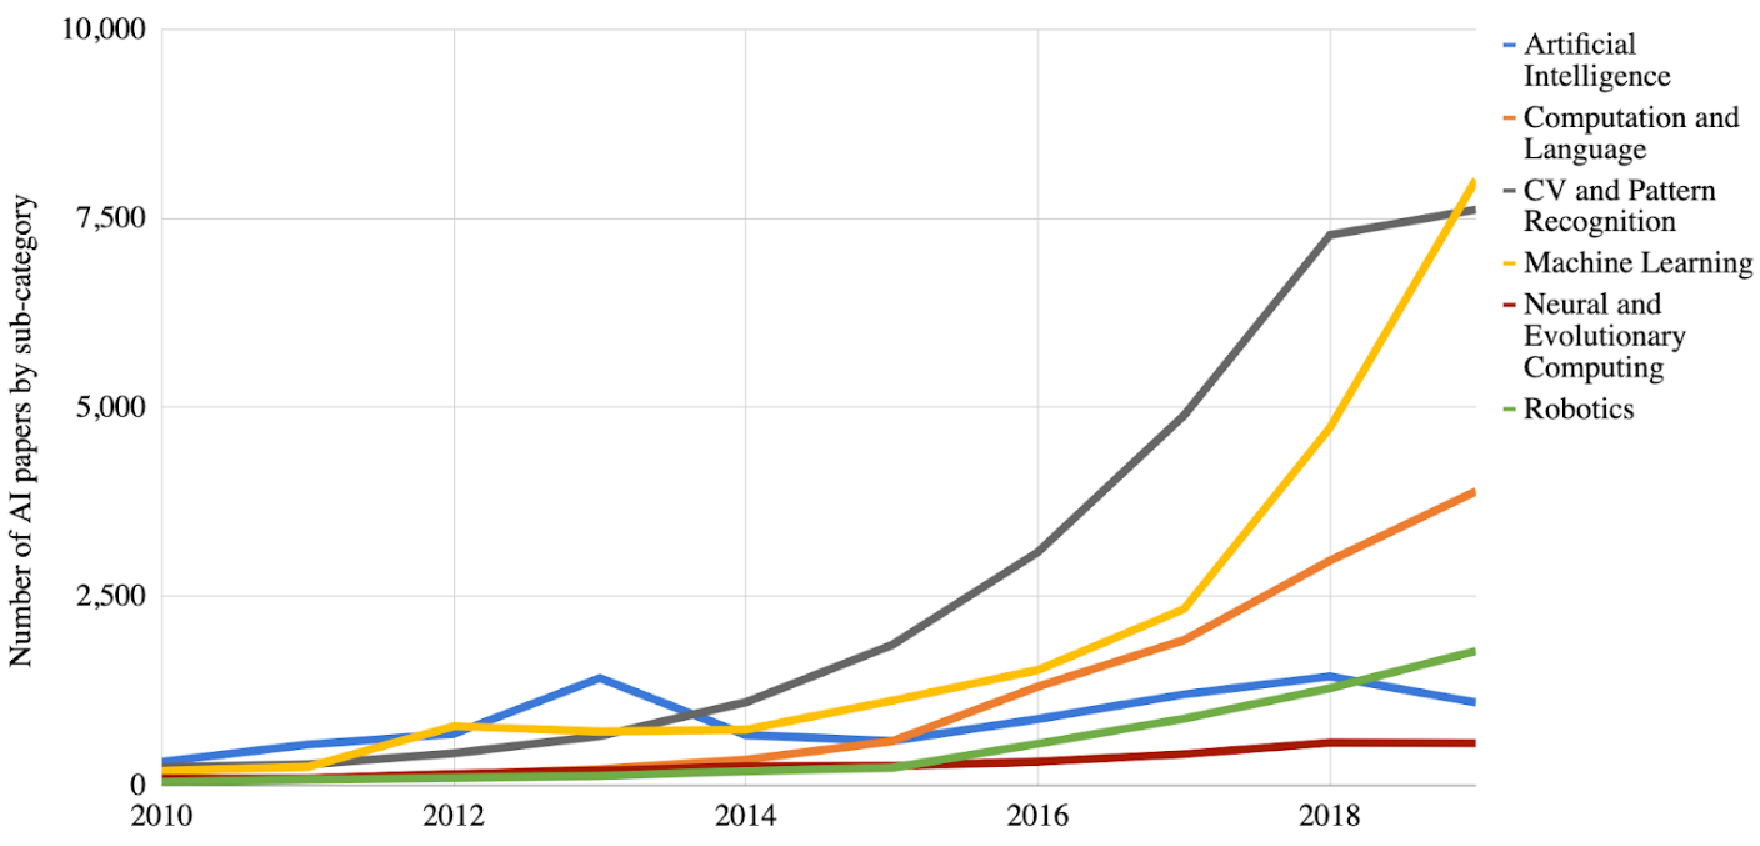
\includegraphics[width=0.8\textwidth]{diagrams/6-cnn/papers.pdf}
    \caption[The number of artificial intelligence papers submitted to arXiv]
    {The number of artificial intelligence papers submitted to arXiv, broken down by sub-category.
        Note the particularly large increase in Computer Vision (CV) and pattern recognition
        papers. Figure taken from \ReferenceRef{perrault2019}.}
    \label{fig:papers}
\end{figure}

In 2016 the \nova experiment applied a CNN to the task of classifying the interaction type of
events within their sampling calorimeter detector~\cite{aurisano2016}. Two views of raw detector
data were used as input to train a network based on the popular GoogLeNet
architecture~\cite{szegedy2015} (discussed in \SectionRef{sec:cnn_theory_conv}). Further \nova
iterations have since been applied to both the classification of individual energy deposit
clusters~\cite{psihas2019} and $\nu_{e}$ and $e^{-}$ energy reconstruction~\cite{baldi2019}.

CNNs have also been applied to liquid argon time-projection chambers. The MicroBooNE
experiment~\cite{acciarri2017_ref} has shown that in addition to classification tasks, the spatial
localisation of single particles within events is possible~\cite{acciarri2017}. Furthermore, the
DUNE collaboration has designed a network to output both the interaction class and counts of
different particle types within an event~\cite{collaboration2020, abi2020}. This approach is
called \emph{multi-task} learning and is discussed in detail within
\SectionRef{sec:cnn_baseline_outputs}.

Applications to water Cherenkov detectors have also been made by both the Daya Bay
experiment~\cite{racah2016} and the KM3NeT/ORCA collaboration~\cite{aiello2020}. Furthermore, a
type of CNN known as a \emph{variational autoencoder} has been shown to approximate the
distribution of simulated water Cherenkov data well~\cite{abhishek2019}. If further such studies
prove successful, this could allow for training on `real' data to mitigate experimental
uncertainties and vastly increase the speed of simulated data generation.

\section{Standard event reconstruction and classification} %%%%%%%%%%%%%%%%%%%%%%%%%%%%%%%%%%%%%%%
\label{sec:cnn_old} %%%%%%%%%%%%%%%%%%%%%%%%%%%%%%%%%%%%%%%%%%%%%%%%%%%%%%%%%%%%%%%%%%%%%%%%%%%%%%

It is essential to outline the standard event reconstruction and classification methods used by
the \chips project until now. This is for two reasons. Firstly, to highlight their main weaknesses
as motivation for the new CNN approach. Secondly, to provide context for the performance
comparisons made in \ChapterRef{chap:results}.

A likelihood method based on that implemented by MiniBooNE~\cite{patterson2009} is used for event
reconstruction, while a simple neural network built using the TMVA package~\cite{hocker2007} is
used for event classification. Both methods are representative of the mainstream approach used by
the majority of water Cherenkov neutrino experiments for event analysis. A prime example is the
fiTQun algorithm developed for the Super-Kamiokande detector, used for both
atmospheric~\cite{jiang2019} and T2K~\cite{missert2017} analyses.

\subsection{Likelihood-based reconstruction} %%%%%%%%%%%%%%%%%%%%%%%%%%%%%%%%%%%%%%%%%%%%%%%%%%%%%
\label{sec:cnn_old_reco} %%%%%%%%%%%%%%%%%%%%%%%%%%%%%%%%%%%%%%%%%%%%%%%%%%%%%%%%%%%%%%%%%%%%%%%%%

The event reconstruction methodology is simple in theory: for a given set of hypothesised charged
particle tracks, the number of Cherenkov photoelectrons and the time at which the first of these
is recorded for each PMT in the detector is predicted. By comparing this prediction with the
measured hit charges and times the likelihood that the given track hypothesis produced the
measured signals can be calculated. The parameters that describe the hypothesised tracks are then
varied until the negative logarithm of the likelihood is minimised, identifying the best-fit
parameters. A brief description of the full procedure is given below, however, for a detailed
description see \ReferenceRef{blake2016} and \ReferenceRef{perch2017}. The full C++ software
implementation can also be found in the repository at \ReferenceRef{chipsreco2020}.

\subsubsection*{Seeding} %%%%%%%%%%%%%%%%%%%%%%%%%%%%%%%%%%%%%%%%%%%%%%%%%%%%%%%%%%%%%%%%%%%%%%%%%

The first stage of event reconstruction is the effective \emph{seeding} of tracks that are then
used in the full likelihood fit. The seeding methods aim to provide a good starting point for the
minimisation, both to increase the efficiency of finding the optimal track parameters and also to
avoid a false local minimum from being returned.

Firstly, the PMT hits are sliced in both space and time. Gaps in the time ordering of hits are
used to separate the event into time slices. Each of these slices then undergoes basic clustering
to remove outlying hits and ensure only the dominant collections of hits are considered. This
procedure involves removing all hits that fall outside of clusters containing at least 50 hits
generated by finding hits that fall within \SI{2}{\text{m}} of each other. Each cleaned slice is
then run through simple geometric vertex finding algorithms to estimate the interaction position
and time, in addition to the initial direction of the track.

A circular \emph{Hough transform} algorithm, traditionally used for water Cherenkov ring finding
is then applied~\cite{illingworth1988}. As output, the voting-based transformation produces a
space within which rings of PMT hits exist as peaks. The track direction values are further
refined using this space before a search for secondary peaks is carried out to indicate if
multiple particles are likely to be involved. This process results in a list of seeds, each with a
score related directly to the height of the associated peak in Hough transform space.

\subsubsection*{Likelihood fit} %%%%%%%%%%%%%%%%%%%%%%%%%%%%%%%%%%%%%%%%%%%%%%%%%%%%%%%%%%%%%%%%%%


Each particle track in a fit hypothesis comprises a vector of parameters $\vec{x}$, containing the
following:
\begin{itemize}
    \item the track interaction vertex position ($x_{0}$, $y_{0}$, $z_{0}$) and time ($t_{0}$);
    \item the initial track direction ($d_{\theta}$, $d_{\phi}$);
    \item the initial kinetic energy of the particle ($E$); and
    \item the particle type (muon, electron or photon).
\end{itemize}
For a photon hypothesis the distance between the interaction vertex and the beginning of the
electromagnetic shower is also included as a parameter.

The hypothesised tracks are then initialised using the list of seeds found in the seeding
procedure in descending order of Hough peak height score. As the seeding algorithms do not
estimate the particle energy, a default value equal to the average particle energy observed within
a sample run through the detector Monte Carlo simulation is assigned. Additionally, constraints
can be placed on a multi-track hypothesis to reduce the number of free parameters.

As an example, consider the NC $\pi^{0}$ case, where a multi-track two-photon hypothesis is used.
Firstly, the initial parameters for the two photons are assigned from the two highest-scoring
seeds from the seeding procedure. Secondly, the vertex position for both tracks is constrained to
remain the same, and the directions and energies are set to be constrained by the invariant mass
of the $\pi^{0}$.

In its simplest form the likelihood $\mathcal{L}(\vec{x})$, is a simple product of two terms:
\begin{equation} % LIKELIHOOD EQUATION %
    \mathcal{L}(\vec{x})=\mathcal{L}_{unhit}(\vec{x})\mathcal{L}_{hit}(\vec{x})=
    \prod_{unhit}P_{unhit}(\vec{x})\prod_{hit}P_{charge}(\vec{x})P_{time}(\vec{x}),
    \label{eq:likelihood}
\end{equation}
where the first ($unhit$) term gives the likelihood that the hypothesis $\vec{x}$ will not predict
a hit on the PMTs that do not have a measured hit, and the second ($hit$) term gives the
likelihood that $\vec{x}$ produces the observed photoelectrons and hit times on the measured hit
PMTs. 

By considering the negative logarithm of the likelihood the computation can be simplified into a
sum of logarithms over the PMTs, such that
\begin{equation} % LIKELIHOOD SUM PMTS EQUATION %
    -\log\mathcal{L}(\vec{x})=
    -\sum_{unhit}\log(P_{unhit}(\vec{x}))
    -\sum_{hit}\log(P_{charge}(\vec{x}))
    -\sum_{hit}\log(P_{time}(\vec{x})).
    \label{eq:likelihood_sum}
\end{equation}
This form has the effect of separating the charge (number of photoelectrons) and time prediction
components, which can then be dealt with separately computationally. In the actual likelihood
calculation the $P_{unhit}(\vec{x})$ and $P_{charge}(\vec{x})$ components are combined, where the
probability of an unhit PMT is treated as a PMT with an observed charge equal to zero.

The Minuit2 algorithm contained within the ROOT software package~\cite{brun1997} is used for the
minimisation process. At each iteration, the charge and hit time predictions are made, and the
negative logarithm of the likelihood is calculated. The track parameters are then varied to
minimise the likelihood before the next iteration begins. Through a series of stages, each fixing
and freeing specific parameters, the minimisation process converges to the best-fit parameters for
the given hypothesis. This procedure typically takes two minutes on a standard batch farm
computing node.

\subsubsection*{Downsides} %%%%%%%%%%%%%%%%%%%%%%%%%%%%%%%%%%%%%%%%%%%%%%%%%%%%%%%%%%%%%%%%%%%%%%%

The charge and hit time predictions and their associated likelihood contributions depend on a
series low-level inputs. Generally, these inputs describe how Cherenkov light is emitted from
specific particles and how it propagates through the detector to be detected by the PMTs. Examples
of these inputs include:
\begin{itemize}
    \item the number of Cherenkov photons emitted by a particle of a specific type and energy;
    \item the fraction of Cherenkov light emitted at each step along a specific particle's track
          length;
    \item the angular distribution of Cherenkov photon emission for each type of particle;
    \item the survival probability of photons within the detector medium as a function of distance
          and energy;
    \item a detailed description of the PMT positions and directions;
    \item the angular efficiency of each PMT relative to the incident photon angle; and
    \item the probability of a measured charge given the predicted number of photoelectrons (see
          \FigureRef{fig:digi_likelihood}).
\end{itemize}

The above list demonstrated a fundamental problem with the likelihood-based approach. Namely, it
is only dependent on a finite list of inputs that must be implemented in software. If a physical
process is overlooked, then the algorithm has access to a reduced amount of information with which
to predict the PMT hit charges and times, impacting the performance of the best-fit track
parameters. Additionally, the large amount of effort required to implement and correctly model
each input can make a likelihood-based approach time-consuming.

Moreover, the likelihood-based approach requires a predefined track hypothesis per fit. This
restriction is at odds with the broad array of neutrino events expected within \chips detector
modules. Many possible combinations of final state particles are possible, making the
implementation of an approach where all possible events are considered, challenging. For example,
the very similar Super-Kamiokande fiTQun algorithm attempts multiple fits for each event,
sequentially adding charged particles to the hypothesis until the best-fit is found. This
technique not only vastly increases the time required to analyse a single event, but can never be
fully rigorous as it still ignores some scenarios.

\subsection{Event classification}%%%%%%%%%%%%%%%%%%%%%%%%%%%%%%%%%%%%%%%%%%%%%%%%%%%%%%%%%%%%%%%%%
\label{sec:cnn_old_pid} %%%%%%%%%%%%%%%%%%%%%%%%%%%%%%%%%%%%%%%%%%%%%%%%%%%%%%%%%%%%%%%%%%%%%%%%%%

As the standard event reconstruction is based on the calculation of a likelihood (analogous to a
goodness-of-fit), the likelihood ratio between different hypotheses can be used for event
classification tasks. Additional hand-engineered features derived from the reconstruction outputs
are also found to have power in classifying the event type.

Two simple neural networks are used, the first for CC $\nu_{e}$ - CC $\nu_{\mu}$ separation and
the second for CC $\nu_{e}$ - NC separation. Both contain a single hidden layer (as described in
the following \SectionRef{sec:cnn_theory}) with the number of neurons equal to the number of input
parameters plus five. Output variables from both a single electron track and single muon track
hypothesis fit are used for both networks, including:
\begin{itemize}
    \item the $\Delta\log\mathcal{L}$ between $e$ and $\mu$ hypothesis for both time and charge
          components;
    \item the total number of hit PMTs ($N_{hits}$) and total collected charge;
    \item $\frac{\Delta\log\mathcal{L}_{charge}}{N_{hits}}$;
    \item the fraction of hits inside, within, and outside the ring for both the $e$ and $\mu$
          hypotheses;
    \item the fraction of predicted charge outside the ring for both the $e$ and $\mu$ hypotheses;
    \item the ratio of the total predicted charged to the total measured charge for both the $e$
          and $\mu$ hypothesis;
    \item the ratio of the reconstructed energy to the total measured charge for both the $e$ and
          $\mu$ hypotheses;
    \item the reconstructed track direction under the $e$ hypothesis;
    \item the fraction of hits in the downstream half of the detector;
    \item the number of seeds generated by the Hough transform seeding algorithm; and
    \item the peak height score of the first and last seeds found by the Hough transform seeding
          algorithm.
\end{itemize}

A sample of CC $\nu_{e}$ and CC $\nu_{\mu}$ beam events characteristic of those expected to be
seen within \chipsfive are used to train the first classifier, and a corresponding sample of CC
$\nu_{e}$ and NC events for the second. The output values from both networks can then be used to
select CC $\nu_{e}$ events from the background. Note that only the selection of CC $\nu_{e}$
events has been implemented, no CC $\nu_{\mu}$ selection has been developed.

The principal limitation of this approach is that the input features are restricted to those that
have been imagined (requiring extensive domain knowledge) and then implemented in software. The
current list is undoubtedly non-exhaustive of all the possible variables and combinations of
variables that can, in theory, be used for discrimination between events. Additionally, any
systematic uncertainties in the likelihood-based reconstruction and, therefore, input variables to
the neural networks, can lead to incorrect classification of events.

\section{The theory of neural networks} %%%%%%%%%%%%%%%%%%%%%%%%%%%%%%%%%%%%%%%%%%%%%%%%%%%%%%%%%%
\label{sec:cnn_theory} %%%%%%%%%%%%%%%%%%%%%%%%%%%%%%%%%%%%%%%%%%%%%%%%%%%%%%%%%%%%%%%%%%%%%%%%%%%

There are many machine learning techniques: linear regression, logistic regression, k-nearest
neighbours, decision trees, random forests, support vector machines, amongst others, all of which
learn to make predictions about data. However, none has been as successful, especially in recent
years, as the deep neural network. As both the size of datasets and the amount of available
computing power has increased, deep neural networks have proved incredibly powerful for many
tasks, as they are well suited to this paradigm.

Here we discuss the application of neural networks for \emph{supervised learning}, one of two
broad machine learning categories concerned with using labelled example data to train algorithms.
The other broad category of \emph{unsupervised learning}, where the properties of the dataset are
inferred without labelled data is not discussed, however, will be used for network
\emph{explainability} in \SectionRef{sec:results_explain}.

\subsection{Neural network basics} %%%%%%%%%%%%%%%%%%%%%%%%%%%%%%%%%%%%%%%%%%%%%%%%%%%%%%%%%%%%%%%
\label{sec:cnn_theory_basics} %%%%%%%%%%%%%%%%%%%%%%%%%%%%%%%%%%%%%%%%%%%%%%%%%%%%%%%%%%%%%%%%%%%%

A neural network is a type of algorithm inspired by the repeating cell structure of neurons within
our brains. The basic building block of a neural network is a \emph{neuron}, which takes a vector
of $k$ inputs $\vec{x}=(x_{1}, x_{2},\dots,x_{k})$ and outputs a scalar $a(\vec{x})$. Individual
neurons are arranged into layers, with the input of one layer being the output from the previous
layer. The first layer is commonly referred to as the \emph{input layer}, the middle layers as
\emph{hidden layers}, and the final layer as the \emph{output layer}, as illustrated in
\FigureRef{fig:network}. In general, this simple neural network structure is referred to as
\emph{fully-connected}, as all the neurons in each layer have connections to all the neurons in
the previous and following layers.

\begin{figure} % BASIC NETWORK DIAGRAM %
    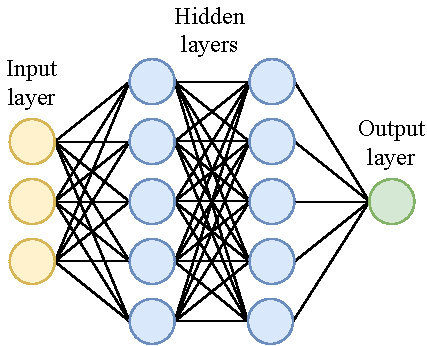
\includegraphics[width=0.6\textwidth]{diagrams/6-cnn/network.pdf}
    \caption[Illustration of a simple neural network]
    {Illustration of a simple neural network. There is a single input layer (yellow), two hidden
        layers (blue), and an output layer (green). Each node corresponds to a neuron except for
        the input layer.}
    \label{fig:network}
\end{figure}

Input variables (traditionally hand-engineered features extracted from the raw data) are passed
into the network via the input layer. Any number of hidden layers containing any number of neurons
can then follow. The neurons contained within these layers are trained so that collectively their
$a(\vec{x})$ functions solve the task at hand. For a regression task, the output layer returns a
continuous decimal value. Conversely, for a classification task, a probability value between zero
and one is output for each class. The forward passing of information from one layer to the next is
why neural networks can also be referred to as \emph{feed-forward graphs}.

For a neuron $i$, $a_{i}(\vec{x})$ can be decomposed into a neuron specific linear operation,
followed by a non-linear operation which is the same across all neurons. The linear operation
consists of the dot product of the input vector $\vec{x}$ with a vector of weights
$\vec{w}^{(i)}=(w_{1}^{(i)}, w_{2}^{(i)},\dots,w_{k}^{(i)})$, plus a bias term $b^{(i)}$:
\begin{equation} % NETWORK BASIC EQUATION %
    z^{(i)}=\vec{w}^{(i)}\cdot\vec{x}+b^{(i)}.
    \label{eq:network}
\end{equation}
After applying the non-linear operation $\sigma_{i}$, commonly referred to as the \emph{activation
    function}, the final neuron output can be written as
\begin{equation} % NETWORK ACTIVATION EQUATION %
    a_{i}(\vec{x})=\sigma_{i}(z^{(i)}).
    \label{eq:activation}
\end{equation}

Traditionally, a step-function (for networks called \emph{perceptrons}) was used for the
activation function. However, as is shown in \SectionRef{sec:cnn_theory_training}, a non-zero
gradient (only valid at $x=0$ for a step-function) is required for the practical training of
neural networks. In fact, the choice of activation function can greatly affect how the network
trains and performs.

Therefore, common activation function choices have been the \emph{hyperbolic tangent} and the
\emph{sigmoid} functions, primarily because they are bounded and differentiable at all points.
Recently, the \emph{ReLU} and other similar functions have become popular, mainly due to their
avoidance of \emph{vanishing} gradients which occur when the tanh and sigmoid functions become
saturated at large values of $x$. All of these functions are shown in \FigureRef{fig:activations}
for reference.

\begin{figure} % ACTIVATIONS DIAGRAM %
    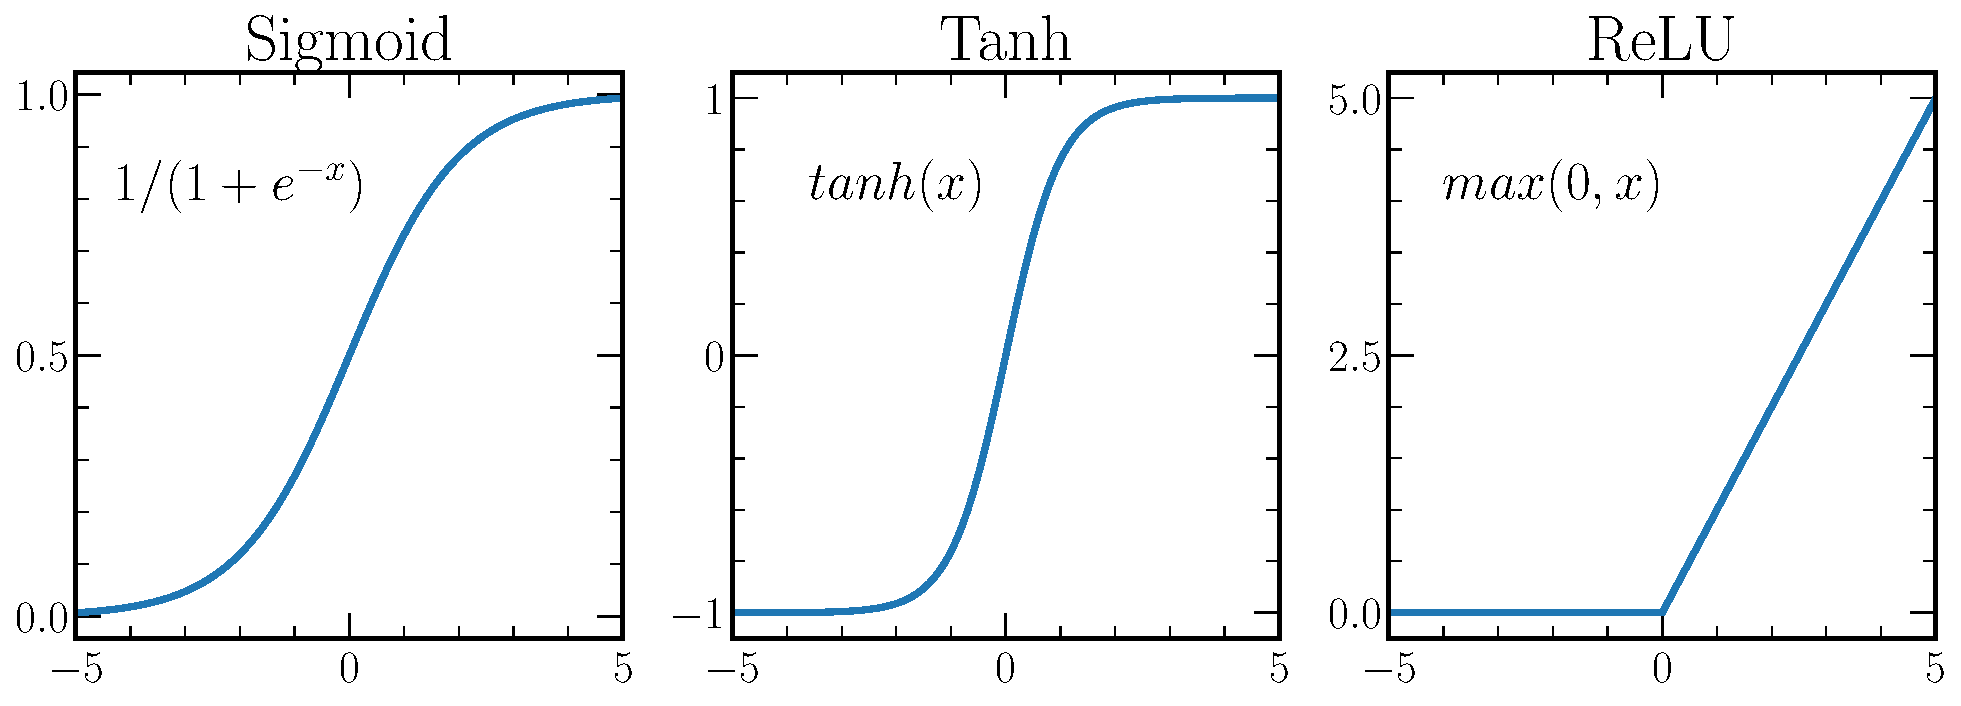
\includegraphics[width=\textwidth]{diagrams/6-cnn/activations.pdf}
    \caption[Common non-linear activation functions]
    {Common non-linear activation functions used for the neurons within neural networks.}
    \label{fig:activations}
\end{figure}

\subsection{Training neural networks} %%%%%%%%%%%%%%%%%%%%%%%%%%%%%%%%%%%%%%%%%%%%%%%%%%%%%%%%%%%%
\label{sec:cnn_theory_training} %%%%%%%%%%%%%%%%%%%%%%%%%%%%%%%%%%%%%%%%%%%%%%%%%%%%%%%%%%%%%%%%%%

Supervised neural network training uses labelled example data to iteratively find the optimal
weights and biases (the network parameters) to maximise output performance. A \emph{loss function}
$E(\vec{w})$, is defined to quantify the difference between the network output and truth label for
each example, where $\vec{w}$ is the vector of network parameters. For a given input example
$(\vec{x}_{i}, y_{i})$, with $\vec{x}_{i}$ being the input parameters and $y_{i}$ the known truth
label, the network generates an output $\hat{y}_{i}(\vec{w})$. Using this notation, we can
construct loss functions suitable for different tasks.

In the case of simple binary classification the most commonly used function is the \emph{binary
cross-entropy}, where
\begin{equation} % BINARY CROSS-ENTROPY EQUATION %
    E(\vec{w})=
    -\displaystyle\sum_{i=1}^{n}y_{i}\log\hat{y}_{i}(\vec{w})+
    (1-y_{i})\log[1-\hat{y}_{i}(\vec{w})],
    \label{eq:binary_cross_entropy}
\end{equation}
with the number of examples given by $n$. For a classification task where the number of classes is
greater than two $y$ can instead take on $M$ values. In this case we redefine each example so that
$y$ is instead a vector $y_{im}$, such that
\begin{equation} % ONE-HOT EQUATION %
    y_{im}=
    \begin{cases}
        1 & \text{if $y_{i}=m$,} \\
        0 & \text{otherwise.}   \\
    \end{cases}
\end{equation}
This is commonly named a \emph{one-hot} vector. The cross-entropy then becomes the
\emph{categorical cross-entropy}, given by
\begin{equation} % CATEGORICAL CROSS-ENTROPY EQUATION %
    E(\vec{w})=
    -\displaystyle\sum_{i=1}^{n}\displaystyle\sum_{m=0}^{M-1}y_{im}\log\hat{y}_{im}
    (\vec{w})+(1-y_{im})\log[1-\hat{y}_{im}(\vec{w})].
    \label{eq:categorical_cross_entropy}
\end{equation}
For a regression task predicting a continuous output variable, the \emph{mean-squared error} is
most often used as the loss function, with
\begin{equation} % MEAN-SQUARED ERROR LOSS EQUATION %
    E(\vec{w})=
    \frac{1}{n}\displaystyle\sum_{i=1}^{n}(y_{i}-
    \hat{y}_{i}(\vec{w}))^{2}.
    \label{eq:mse}
\end{equation}

To find the optimal network parameters for the given task the loss function output (the
\emph{loss}) is iteratively minimised until it converges to the minimum (or in reality a local
minimum that performs well). This is done by updating the network parameters at each iteration
$t$, to move in the direction of the loss gradient, using the update rule
\begin{equation} % UPDATE EQUATION %
    \vec{w}_{t+1}=\vec{w}_{t}-\eta_{t}\nabla_{\vec{w}}E(\vec{w}),
    \label{eq:update_rule}
\end{equation}
where $\eta_{t}$ is the \emph{learning rate} which determines the size of the step taken at each
iteration. This methodology is known as \emph{gradient descent} and is illustrated in
\FigureRef{fig:gradient_descent}.

\begin{figure} % GRADIENT DESCENT DIAGRAM %
    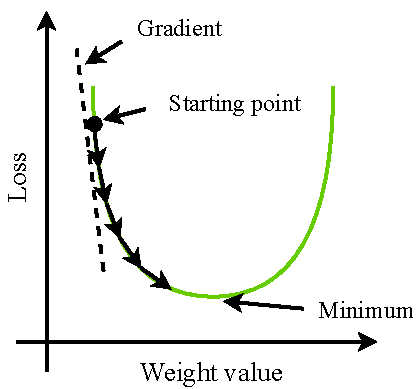
\includegraphics[width=0.5\textwidth]{diagrams/6-cnn/gradient_descent.pdf}
    \caption[Illustrative diagram of the gradient descent process]
    {Illustrative diagram of the gradient descent procedure. Shown is the case for a loss function
        dependent on a single weight.}
    \label{fig:gradient_descent}
\end{figure}

Therefore, to use gradient descent, we require that the gradient of the loss function with respect
to the parameters of the network can be calculated. Doing this for each parameter at every
iteration would render neural networks impossible to train due to the vast computational
requirements. Instead, an innovative application of the chain rule, in an algorithm called
\emph{backpropagation} is used~\cite{werbos1974}. Here we follow the derivation of the four main
backpropagation equations given in \ReferenceRef{mehta2019}.

For a network containing $L$ layers, we can index the individual layers using $l=1,\dots,L$. The
weight associated with the connection between the $k$-th neuron in layer $l-1$ and the $j$-th
neuron in layer $l$ can be denoted as $w^{l}_{jk}$, with the bias of the layer $l$ neuron
correspondingly written as $b^{l}_{j}$. The activation of the $j$-th neuron in layer $l$ is then
related to the outputs from the previous layer by
\begin{equation} % PREVIOUS LAYER EQUATION %
    a^{l}_{j}=\sigma(z^{l}_{j})=\sigma\left(\sum_{k}w^{l}_{jk}a^{l-1}_{k}+b^{l}_{j}\right),
    \label{eq:feedforward}
\end{equation}
where $\sigma$ is the non-linear activation function.

The change in the loss function with respect to the linear weighted sum $z^{L}_{j}$ of the $j$-th
neuron in the last layer $L$, defines the error $\Delta^{L}_{j}$, such that
\begin{equation} % PREVIOUS LAYER EQUATION %
    \Delta^{L}_{j}=\frac{\partial E}{\partial z^{L}_{j}}.
\end{equation}
Using the chain rule and the fact that $a^{L}_{j}=\sigma(z^{L}_{j})$, the error is found to be
equivalent to
\begin{equation} % BACKPROP EQUATION 1 %
    \Delta^{L}_{j}=\frac{\partial E}{\partial a^{L}_{j}}
    \sigma '(z^{L}_{j}),
    \label{eq:backprop_1}
\end{equation}
where $\sigma '(z^{L}_{j})$ denotes the derivative of the non-linear activation function at
$z^{L}_{j}$. This (\EquationRef{eq:backprop_1}) is the first of the backpropagation equations.

The error $\Delta^{l}_{j}$, of the $j$-th neuron in layer $l$ can be expressed in terms of the
error in the following layer $l+1$, by using
\begin{equation} % BACKPROP EQUATION 3 %
    \begin{aligned}[b]
        \Delta^{l}_{j} &=\frac{\partial E}{\partial z^{l}_{j}}, \\
        &=\sum_{k}\frac{\partial E}{\partial z^{l+1}_{k}}
        \frac{\partial z^{l+1}_{k}}{\partial z^{l}_{j}}, \\
        &=\sum_{k}\Delta^{l+1}_{k}\frac{\partial z^{l+1}_{k}}{\partial z^{l}_{j}}, \\
        &=\left(\sum_{k}\Delta^{l+1}_{k}w^{l+1}_{kj}\right)\sigma '(z^{l}_{j}).
        \label{eq:backprop_2}
    \end{aligned}
\end{equation}
The chain rule has again been used in addition to the fact that
\begin{equation}
    z^{l+1}_{k}=\sum_{j}w^{l+1}_{kj}\sigma(z^{l}_{j})+b^{l+1}_k,
\end{equation}
to give the second of the backpropagation equations (\EquationRef{eq:backprop_2}).

As $\partial b^{l}_{j}/\partial z^{l}_{j}=1$, the error can also be viewed as the partial
derivative of the loss function with respect to the bias, such that
\begin{equation} % BACKPROP EQUATION 2 %
    \Delta^{l}_{j}=\frac{\partial E}{\partial z^{l}_{j}}
    =\frac{\partial E}{\partial b^{l}_{j}}\frac{\partial b^{l}_{j}}{\partial z^{l}_{j}}
    =\frac{\partial E}{\partial b^{l}_{j}},
    \label{eq:backprop_3}
\end{equation}
giving the third of the backpropagation equations (\EquationRef{eq:backprop_3}).

The final backpropagation equation is given by the differential of the cost function with respect
to the weight $w^{l}_{jk}$, which can be written as
\begin{equation} % BACKPROP EQUATION 4 %
    \frac{\partial E}{\partial w^{l}_{jk}}
    =\frac{\partial E}{\partial z^{l}_{j}}\frac{\partial z^{l}_{j}}{\partial w^{l}_{jk}}
    =\Delta^{l}_{j}a^{l-1}_{k}.
    \label{eq:backprop_4}
\end{equation}

The full backpropagation algorithm then proceeds as follows:
\begin{enumerate}
    \item After calculating the activations $a^{1}_{j}$ for all neurons in the input layer, use
          the feed-forward architecture of the network to calculate all the activations at every
          layer using \EquationRef{eq:feedforward}.
    \item Use \EquationRef{eq:backprop_1} to calculate the errors of the last layer neurons,
          requiring both the derivatives of the loss and activation functions.
    \item Use \EquationRef{eq:backprop_2} to `backpropagate' the error through the network from
          the last layer to the input layer, calculating all $\Delta^{l}_{j}$ values.
    \item Calculate the gradient of the loss function for all the weights and biases using
          \EquationRef{eq:backprop_3} and \EquationRef{eq:backprop_4}.
\end{enumerate}

A single activation finding \emph{forward pass} followed by a single error propagating
\emph{backward pass} is all that's required to calculate the gradients for all weights and biases
within the network. This incredibly efficient procedure allows for the use of gradient descent
when training neural networks.

\subsection{Convolutional neural networks} %%%%%%%%%%%%%%%%%%%%%%%%%%%%%%%%%%%%%%%%%%%%%%%%%%%%%%%
\label{sec:cnn_theory_conv} %%%%%%%%%%%%%%%%%%%%%%%%%%%%%%%%%%%%%%%%%%%%%%%%%%%%%%%%%%%%%%%%%%%%%%

The broad category of deep learning covers multiple neural network techniques spanning a range of
application fields such as computer vision, speech recognition, and natural language processing.
By stacking many layers on top of each other to form a `deep' network, these methods offer
increased problem solving capacity by allowing higher-order non-linear functions to form
throughout the network. As a direct consequence, instead of requiring hand-engineered features as
input, deep networks can learn to extract the most powerful features for a given task from raw
data. Here we outline just the specific deep learning technique used in this work; the CNN.

\subsubsection*{CNN operations} %%%%%%%%%%%%%%%%%%%%%%%%%%%%%%%%%%%%%%%%%%%%%%%%%%%%%%%%%%%%%%%%%%

At their core, CNNs make use of a mathematical operation called \emph{convolution}, which either
entirely or in part replaces the simple vector multiplication seen in the fully-connected networks
of \SectionRef{sec:cnn_theory_basics}. This difference makes CNNs incredibly powerful for
applications with grid-like input data such as computer vision tasks.

Using standard CNN terminology, the discrete convolution between the \emph{input} $x$, and the
\emph{kernel} $w$, is given by
\begin{equation}
    f_{i}=(x*w)_{i}=\sum^{\infty}_{j=-\infty}x_{j}w_{i-j},
    \label{eq:convolution}
\end{equation}
where $i$ and $j$ denote the set of discrete values and $f$ is commonly referred to as the
\emph{feature map}. In typical applications, the input is a two-dimensional array $X$. Therefore,
both the kernel $W$, and the resulting feature map $F$, also become two-dimensional. In this case
the convolution operation becomes
\begin{equation}
    F_{i}=(X*W)_{i,j}=\sum_{m}\sum_{n}X_{i+m,j+n}W_{m,n},
    \label{eq:conv}
\end{equation}
where the infinite sum in \EquationRef{eq:convolution} has been replaced with a discrete sum over
two-dimensional elements. Analogous to the simple neural network weights $\vec{w}$, first
described in \EquationRef{eq:network}, the elements of $W_{m,n}$ are trained to minimise the loss,
with the output feature maps passed through a non-linear activation function at each layer.

To illustrate the convolution operation, \FigureRef{fig:conv_input} displays examples of a $4
\times 4$ input grid and a $3 \times 3$ kernel. The output feature map is generated by sliding the
kernel across both dimensions of the input grid, summing the products of all associated elements
at each step according to \EquationRef{eq:conv}, as shown in \FigureRef{fig:conv_operation}.

\begin{figure} % CONV INPUTS DIAGRAM %
    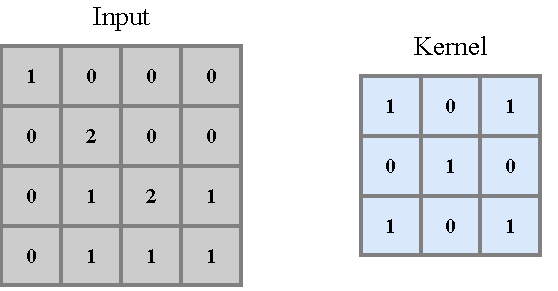
\includegraphics[width=0.7\textwidth]{diagrams/6-cnn/conv_input.pdf}
    \caption[Example of a Convolutional Neural Network input grid and kernel]
    {Example of an input grid (left) and kernel (right). The specific kernel shown is sensitive to
        x-shaped features}
    \label{fig:conv_input}
\end{figure}

\begin{figure} % CONV OPERATION DIAGRAM %
    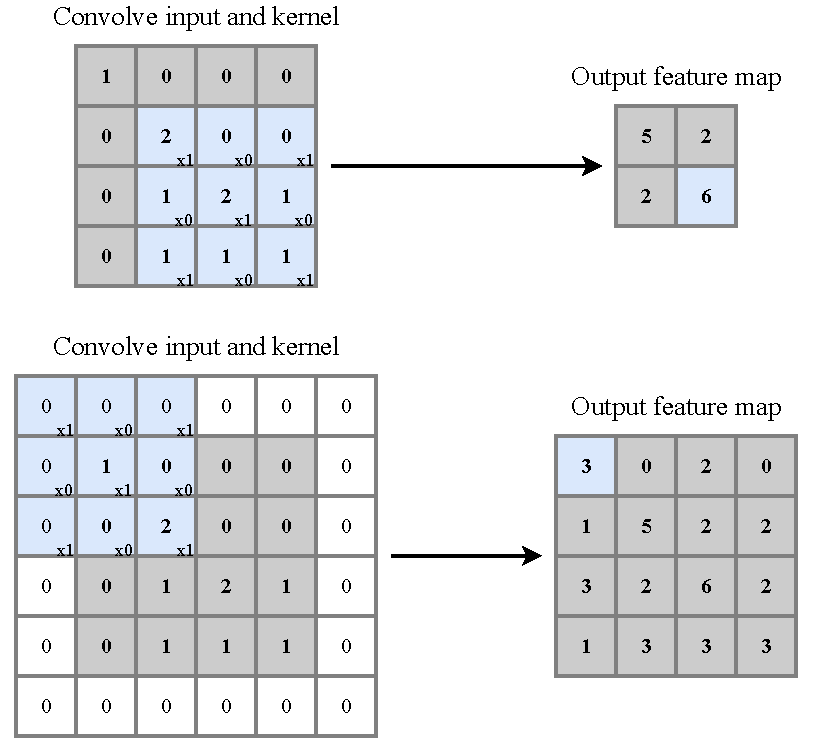
\includegraphics[width=0.8\textwidth]{diagrams/6-cnn/conv_operation.pdf}
    \caption[Example of a convolution operation]
    {Example of a $\text{stride}=1$ convolution operation involving the input grid and kernel from
        \FigureRef{fig:conv_input}. Both the operation for the case of \emph{valid} (top) and
        \emph{same} (bottom) padding are shown. The blue square in the top-left of the output
        feature maps indicates the output generated from the specific operation shown on the left,
        also in blue.}
    \label{fig:conv_operation}
\end{figure}

Two additional parameters impacting the feature map output size are introduced in
\FigureRef{fig:conv_operation}. The \emph{stride} and \emph{padding}. The stride $S$, governs how
far the kernel moves at each step while the padding $P$, decides how the input grid is padded with
zeros around its border. If $L$ is the size of the input (both height and width) and $K$ is the
kernel size, the output feature map size $O$, is given by
\begin{equation}
    O=\frac{(L-K+2P)}{S}+1.
    \label{eq:conv_size}
\end{equation}

The other essential operation used within CNNs is pooling. Pooling layers coarse-grain the spatial
information of the input to reduce the number of network parameters. \emph{Max pooling} or
\emph{average pooling} are the two common ways this is achieved. In both cases, the input is first
divided into rectangular regions, and then either the maximum or average value of the region is
returned as output, for max or average pooling, respectively. Both pooling procedures are
illustrated in \FigureRef{fig:pooling}.

\begin{figure} % POOLING DIAGRAM %
    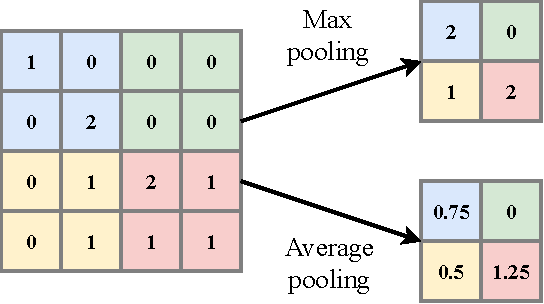
\includegraphics[width=0.7\textwidth]{diagrams/6-cnn/pooling.pdf}
    \caption[Example of pooling operation]
    {Example of both a max and average $2 \times 2$ pooling operation with $\text{stride}=2$.}
    \label{fig:pooling}
\end{figure}

Taking inspiration from how neurons behave in the visual cortex of animals~\cite{lecun2015}, small
kernels are typically used to only scan over a small patch of the input at a time. Combined with
the loss of absolute position information from pooling, a key feature of CNNs is highlighted. They
exhibit translational invariance and respect the local structure contained within the input. In
simpler terms, they do not care wherein the input image a particular feature exists, just that it
exists.

\subsubsection*{CNN architectures} %%%%%%%%%%%%%%%%%%%%%%%%%%%%%%%%%%%%%%%%%%%%%%%%%%%%%%%%%%%%%%%

In 2012 the AlexNet CNN lowered the error rate of the ubiquitous ImageNet classification
task~\cite{deng2009} from 28\% to 16\%~\cite{krizhevsky2012}. Since this breakthrough, the
standard CNN has adopted a similar architecture to AlexNet. Multiple convolutional layers are
stacked on top of each other, periodically interspersed with pooling layers. Once the output
feature map size no longer allows for additional pooling, one or more fully-connected layers are
appended before the output layer, as is illustrated in \FigureRef{fig:conv_diagram}.

\begin{figure} % CONV DIAGRAM %
    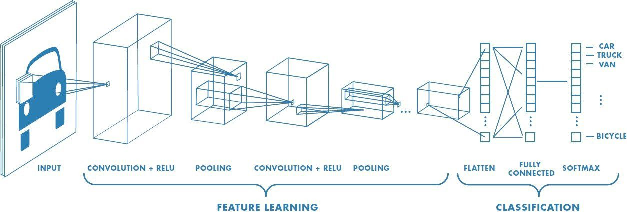
\includegraphics[width=\textwidth]{diagrams/6-cnn/conv_diagram.pdf}
    \caption[Illustration of a typical Convolutional Neural Network architecture]
    {Illustration of a typical CNN architecture containing convolutional, pooling, and
        fully-connected layers before the final output layer. Figure taken from
        \ReferenceRef{convarch2020}.}
    \label{fig:conv_diagram}
\end{figure}

Led primarily by large research teams at the technology giants, improvements upon this standard
architecture have since been made. Initially, this process involved the addition of extra
convolutional layers to form deeper and deeper networks, as was done by the VGG architecture in
2014~\cite{simonyan2014}. Another approach was the introduction of the \emph{inception module}
within the GoogLeNet~\cite{szegedy2015} architecture, allowing for different feature scales to be
considered.

ResNet introduced residual connections in 2016~\cite{he2016_original, he2016_improved}. By adding
connections skipping specific layers, a larger gradient could reach the lower layers of the
network, increasing learning. Recently, the inception module and ResNet concepts have been
combined~\cite{szegedy2016}, and there has been a significant push for efficient rather than just
deeper networks~\cite{sandler2018, tan2019}. The common repeating layer patterns that form the
above networks are shown in \FigureRef{fig:blocks} for reference.

\begin{figure} % BLOCKS DIAGRAM %
    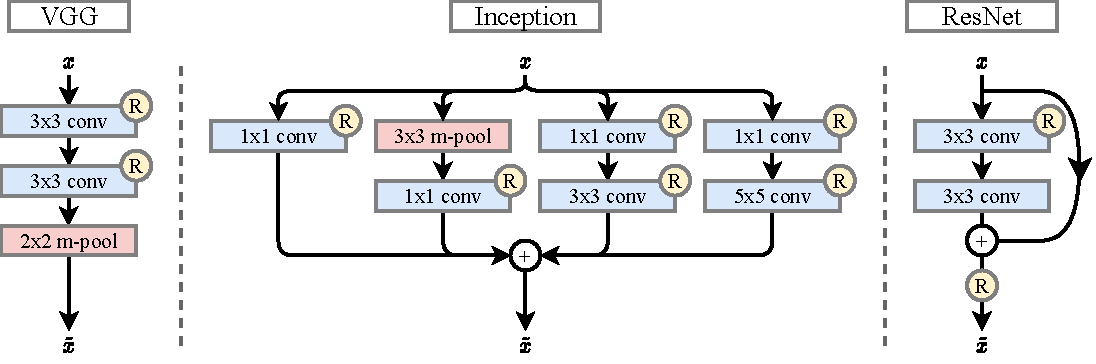
\includegraphics[width=\textwidth]{diagrams/6-cnn/blocks.pdf}
    \caption[Common Convolutional Neural Network architecture blocks]
    {Common repeating layer \emph{blocks} used within CNN architectures, taking $x$ as input and
        producing $\tilde{x}$ as output through operations whose forward pass is shown with the
        arrows. The blue and red boxes represent convolutional (conv) and max-pooling (m-pool)
        layers respectively, with the size of the operation shown. The circular yellow $R$
        indicates the use of the ReLU activation function.}
    \label{fig:blocks}
\end{figure}

\subsection{Regularisation} %%%%%%%%%%%%%%%%%%%%%%%%%%%%%%%%%%%%%%%%%%%%%%%%%%%%%%%%%%%%%%%%%%%%%%
\label{sec:cnn_theory_reg} %%%%%%%%%%%%%%%%%%%%%%%%%%%%%%%%%%%%%%%%%%%%%%%%%%%%%%%%%%%%%%%%%%%%%%%

A key challenge when training supervised machine learning models is ensuring that they can
generalise to new, previously unseen data, not within the training dataset. With networks
typically containing millions of trainable parameters, it can become effortless for them to learn
specific features and noise of the training dataset, rather than generalisable features. This
unwanted learning, called \emph{overfitting}, is ubiquitous when training CNNs. Methods used
within this work to prevent overfitting are outlined below, all of which are commonly referred to
as \emph{regularisation} techniques.

\subsubsection*{Stochastic gradient descent} %%%%%%%%%%%%%%%%%%%%%%%%%%%%%%%%%%%%%%%%%%%%%%%%%%%%%

The gradient descent update equation outlined in \EquationRef{eq:update_rule} updates the network
weights at each training iteration using the gradient calculated over the full training dataset.
This procedure is called \emph{batch training}. It is instead much more common to calculate an
approximation to the complete gradient at each iteration using a \emph{minibatch} of the full
dataset. This is done by considering just a subset of the training data with a size commonly
referred to as the \emph{batch size} and typically equal to a power of two for computational
reasons.

This modification to standard batch training gradient descent is called \emph{stochastic gradient
    descent} as it introduces stochasticity to the training process, providing two main
    advantages. Firstly, the computational time of each iteration is significantly reduced, and
    crucially the memory requirements lowered. Secondly, the addition of minibatch specific noise
    decreases the chance that the minimisation will get stuck in a local minimum suited to
    overfitting the training dataset.

\subsubsection*{Early stopping} %%%%%%%%%%%%%%%%%%%%%%%%%%%%%%%%%%%%%%%%%%%%%%%%%%%%%%%%%%%%%%%%%%

\emph{Early stopping} is another simple regularisation procedure. During training, the training
dataset is commonly iterated over multiple times, with each full iteration called an \emph{epoch}.
By evaluating the error on an independent \emph{validation} dataset at the end of each epoch, the
point at which overfitting starts to occur can be determined, as illustrated in
\FigureRef{fig:early_stopping}. At the determined epoch, the training is stopped to return the
best possible generalised model. In practice, it is common only to stop training after $n$ epochs
have passed with no validation error improvement.

\begin{figure} % EARLY STOPPING DIAGRAM %
    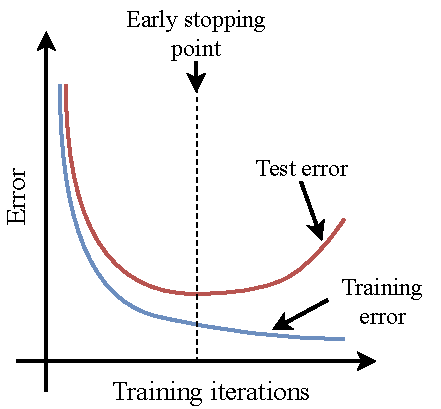
\includegraphics[width=0.5\textwidth]{diagrams/6-cnn/early_stopping.pdf}
    \caption[Illustration of the early stopping procedure]
    {Illustration of the early stopping procedure. Initially both the training and test error
        decrease, but, at some point the test error will start to increase due to overfitting, at
        this point the training is stopped.}
    \label{fig:early_stopping}
\end{figure}

\subsubsection*{Batch normalisation} %%%%%%%%%%%%%%%%%%%%%%%%%%%%%%%%%%%%%%%%%%%%%%%%%%%%%%%%%%%%%

The training of a neural network is found to work best when the inputs of each neuron are centred
on zero with respect to the bias of the neuron. This is because large input values can cause
saturation of the activation function and subsequent vanishing of the associated gradient,
reducing the ability of the network to learn. To counter this, \emph{batch normalisation}
introduces layers that standardise their inputs by using both the mean and variance of each
minibatch~\cite{ioffe2015}. This modification not only speeds up training by preventing the
vanishing of gradients but also reduces overfitting by again using the stochasticity of the
minibatch.

\subsubsection*{Dropout} %%%%%%%%%%%%%%%%%%%%%%%%%%%%%%%%%%%%%%%%%%%%%%%%%%%%%%%%%%%%%%%%%%%%%%%%%

\emph{Dropout} is another simple technique to reduce overfitting~\cite{hinton2012}. At each
training iteration, each neuron has a probability $p_{d}$, to be \emph{dropped out} and ignored
for that iterations calculation. This is illustrated in \FigureRef{fig:dropout}. By ignoring a
subset of neurons at each iteration, it is difficult for the network to form the particularly
strong connections that are usually responsible for overfitting, leading to greater
generalisation.

\begin{figure} % DROPOUT DIAGRAM %
    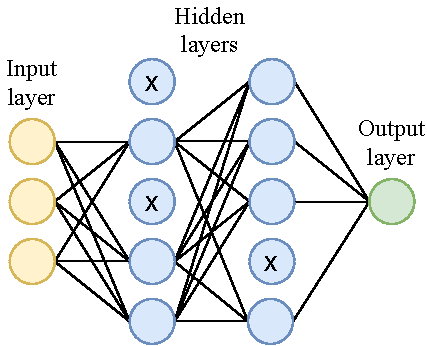
\includegraphics[width=0.6\textwidth]{diagrams/6-cnn/dropout.pdf}
    \caption[Example of dropout applied to a neural network]
    {Example of dropout applied to the network shown in \FigureRef{fig:network}. Neurons are
        randomly \emph{dropped out} and not considered for a training step. This reduces the
        strong connections between neurons that can lead to overfitting.}
    \label{fig:dropout}
\end{figure}

\section{A baseline implementation for CHIPS} %%%%%%%%%%%%%%%%%%%%%%%%%%%%%%%%%%%%%%%%%%%%%%%%%%%%
\label{sec:cnn_baseline} %%%%%%%%%%%%%%%%%%%%%%%%%%%%%%%%%%%%%%%%%%%%%%%%%%%%%%%%%%%%%%%%%%%%%%%%%

The raw output from a water Cherenkov detector, such as those envisioned by the \chips concept, is
a simple image of each event where two channels of information are known for each PMT: the number
of collected photoelectrons, and the associated hit times. Therefore, it is a natural fit to use
CNNs primarily developed for image-based computer vision tasks for \chips event analysis.

For this purpose, a Python-based software package named \emph{chipsnet}~\cite{chipsnet2020} has
been built. By using the high-level \emph{Application Programming Interfaces} (APIs) provided by
the Tensorflow framework (version 2.3.0)~\cite{tf2015}, a full pipeline including data
preparation, network training, and performance evaluation has been implemented. In this section,
the baseline CNN implementation built into chipsnet is outlined. The specific network
implementations described in \SectionRef{sec:cnn_specific} share this common baseline with a few
specific differences.

\subsection{Baseline inputs} %%%%%%%%%%%%%%%%%%%%%%%%%%%%%%%%%%%%%%%%%%%%%%%%%%%%%%%%%%%%%%%%%%%%%
\label{sec:cnn_baseline_inputs} %%%%%%%%%%%%%%%%%%%%%%%%%%%%%%%%%%%%%%%%%%%%%%%%%%%%%%%%%%%%%%%%%%

The primary difficulty in the application of CNNs to \chips is determining how to map an event
captured on a cylindrical surface to a two-dimensional grid. Furthermore, this must be done in
such a way as not to distort the underlying Cherenkov emission topology, which could inhibit
network learning. As a solution, this work takes inspiration and then builds upon the ideas
outlined in \ReferenceRef{theodore2016}. Simply put, an event is mapped onto a two-dimensional
grid as though it is viewed from its estimated interaction vertex position. The primary motivation
behind this is to remove any detector shape effects and to focus on the underlying event topology
and Cherenkov emission profiles.

To estimate each event's interaction vertex position, the top-scoring seed from the seeding
procedure introduced in \SectionRef{sec:cnn_old_reco} is used. This process, unlike the full
likelihood fit, requires no predefined track hypothesis and typically takes under
\SI{0.1}{\text{seconds}} per event on a standard batch farm computing node. The difference between
the true and seed estimated vertex position for a sample of expected beam events are shown in
\FigureRef{fig:explore_true_reco_vtx}. The $x$ component (along the direction of the beam) is
commonly estimated closer to the downstream wall of the detector than reality, however, as the $y$
and $z$ components perpendicular to the beam primarily drive event distortions, the impact on
event topology is small.

\begin{figure} % HOUGH VTX RES DIAGRAM %
    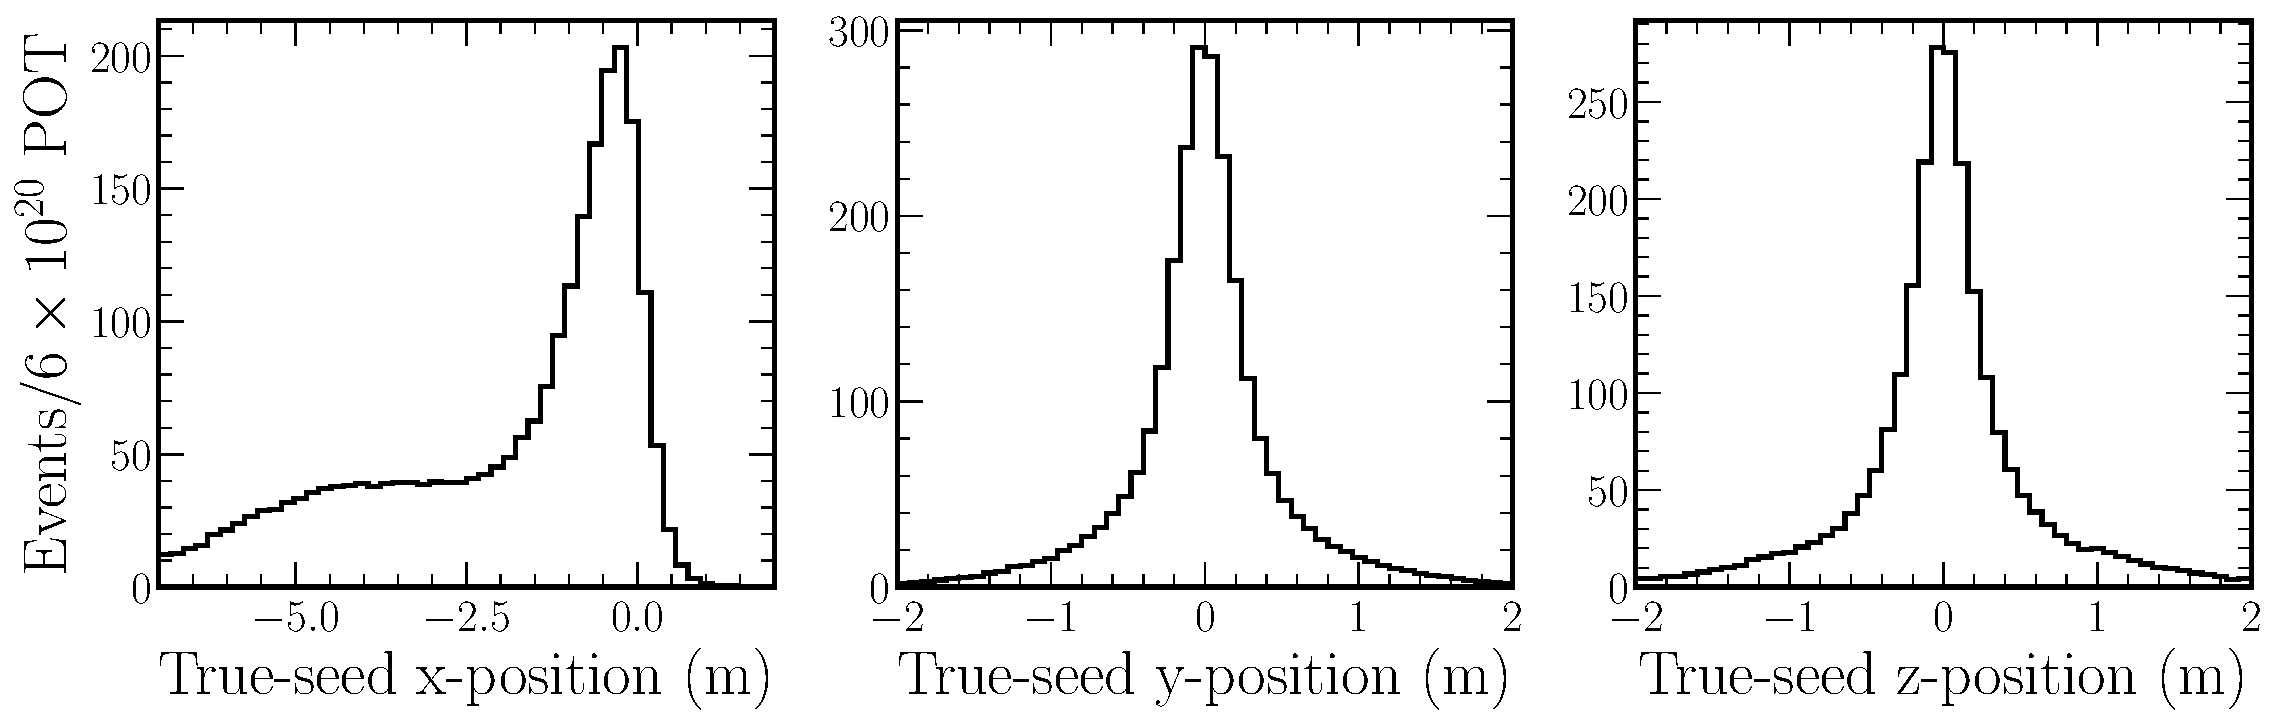
\includegraphics[width=\textwidth]{diagrams/7-results/explore_true_reco_vtx.pdf}
    \caption[Difference between the true and seed estimated vertex position]
    {Difference between the true and seed estimated vertex position, split by component. The large
        negative tail for the $x$ component shows the tendency of the seeding procedure to
        estimate the $x$ component closer to the downstream detector wall than reality.}
    \label{fig:explore_true_reco_vtx}
\end{figure}

Using $\theta$ and $\phi$ components calculated as viewed from the estimated interaction vertex
position facing along the x-axis (downstream), hit PMTs are mapped onto a $64 \times 64$ grid.
This procedure is used to generate two event \emph{maps}. Firstly, a \emph{hit-charge} map where
each grid bin is given by the total collected photoelectrons from all PMTs mapped to that bin.
Secondly, a \emph{hit-time} map where each grid bin is given by the first hit time (in
nanoseconds) across all PMTs mapped to that bin. Each hit-time map is further corrected so that
the first hit time across all bins lies at zero. Note that within this work veto PMTs are ignored
for simplicity.

By design, the Hough transform within the seeding procedure uses the estimated interaction vertex
position to generate the transform space. Therefore, by re-binning the transform space to a $64
\times 64$ grid, a third \emph{hough-height} map is generated for each event. This event map aims
to provide a complementary but different representation of the event where Cherenkov rings are
instead represented as peaks, allowing for additional discriminating features to be learnt.

All three event maps: hit-charge, hit-time, and hough-height are down-sampled using 8-bit encoding
by converting each 32-bit float value to an integer between 0 and 255. Encoding not only
significantly reduces storage requirements but also dramatically increases the speed with which
data can be loaded during training (which turns out to be the primary bottleneck). For each map
type, a range over which to encode from zero up to a \emph{cap-point} is chosen to minimise the
number of bin values that are capped at the maximum encoded value of 255. \TableRef{tab:encoding}
shows the cap-points and the associated percentage of bin values capped for each map type, while
\FigureRef{fig:explore_8_bit_range} shows the distribution of bin values for each event map across
the encoded range.

\begin{table}
    \begin{tabular}{lrr}
        Event map    & Cap-point & Capped percentage \\
        \midrule
        hit-charge   & 25 p.e    & 0.10\%            \\
        hit-time     & 120 ns    & 0.15\%            \\
        hough-height & 3500 p.e  & 0.23\%            \\
    \end{tabular}
    \caption[Table of input event map 8-bit cap-points and percentages]
    {Table showing the input event map cap-points (maximum value of the encoded range) and the
        associated percentage of bin values that are capped at the maximum 8-bit value of 255 as a
        consequence. The cap-points are specifically chosen so that the capped percentage is
        approximately 0.1\%, keeping any information loss small.}
    \label{tab:encoding}
\end{table}

\begin{figure} % 8-BIT DIAGRAM %
    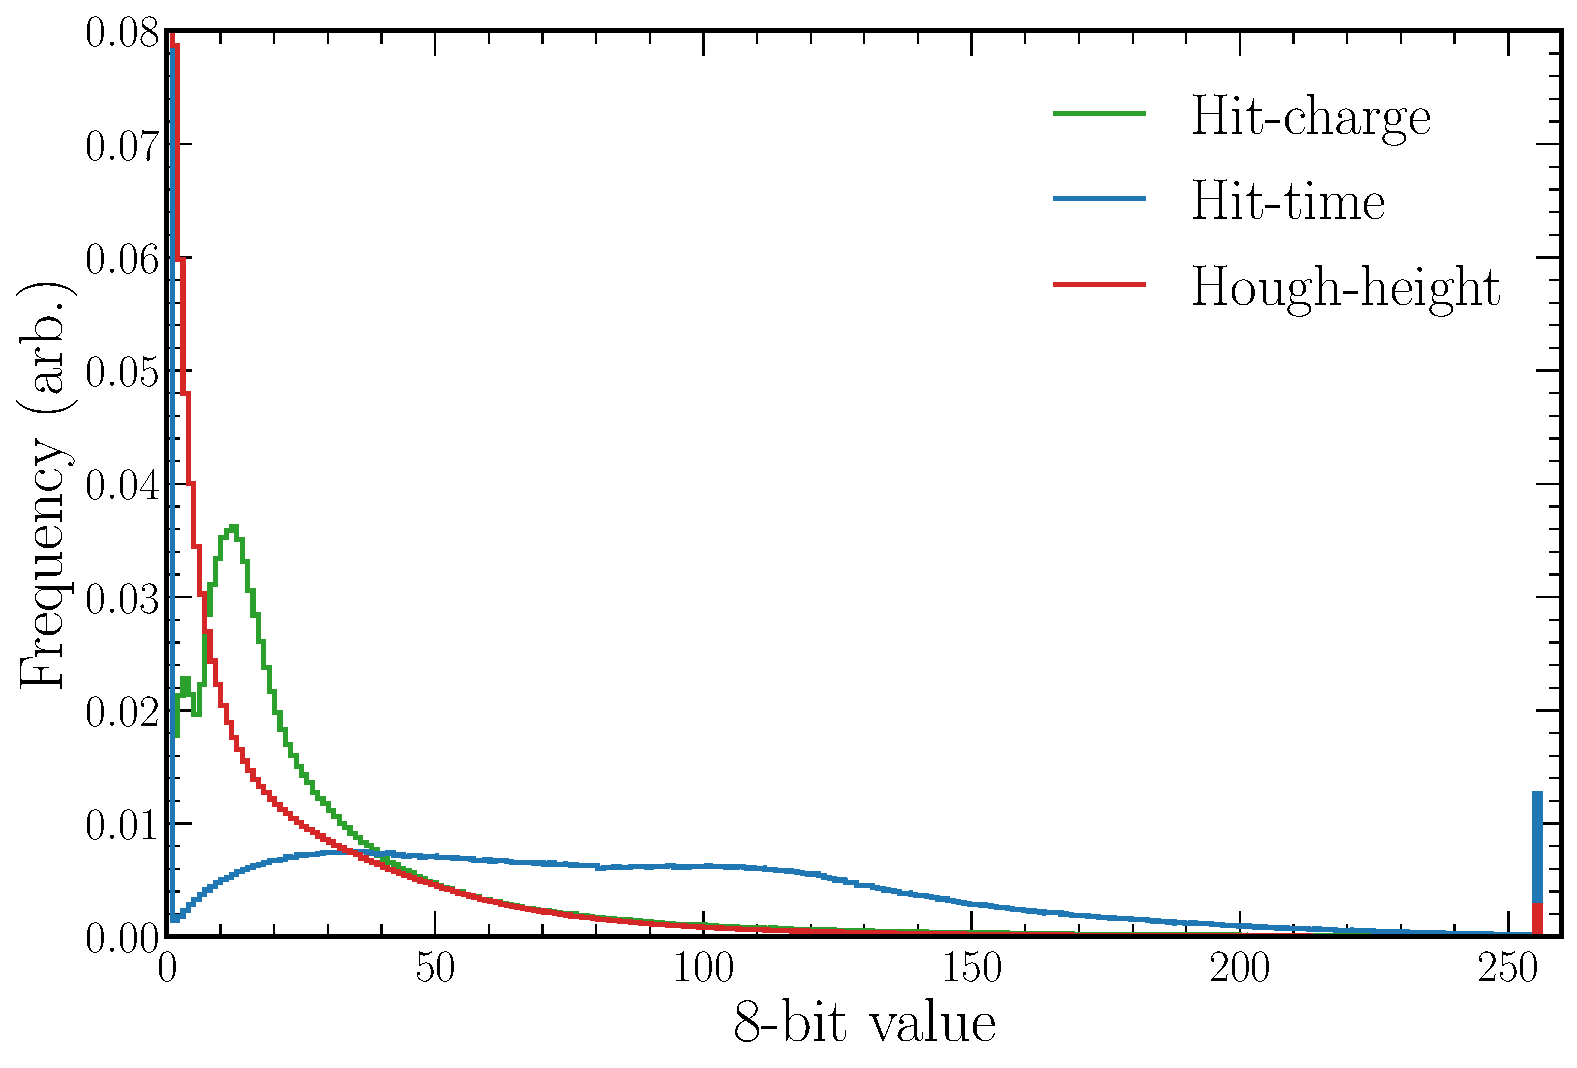
\includegraphics[width=0.7\textwidth]{diagrams/7-results/explore_8_bit_range.pdf}
    \caption[Event map encoded 8-bit distributions]
    {The distribution of encoded 8-bit values for the hit-charge, hit-time and hough-height event
        maps. Note that due to differences in scaling, the values in the bin at an 8-bit value of
        255 do not correspond to those shown in \TableRef{tab:encoding}.}
    \label{fig:explore_8_bit_range}
\end{figure}

Event maps for example events generated using the above procedure are shown in
\FigureRef{fig:explore_nuel_ccres_event} for a CC resonant $\nu_{e}$ event, in
\FigureRef{fig:explore_numu_ccdis_event} for a CC DIS $\nu_{\mu}$ event, in
\FigureRef{fig:explore_nuel_ncdis_event} for a NC DIS event, and in
\FigureRef{fig:explore_cosmic_event} for a cosmic muon event.

\begin{figure} % NUEL EVENT DIAGRAM %
    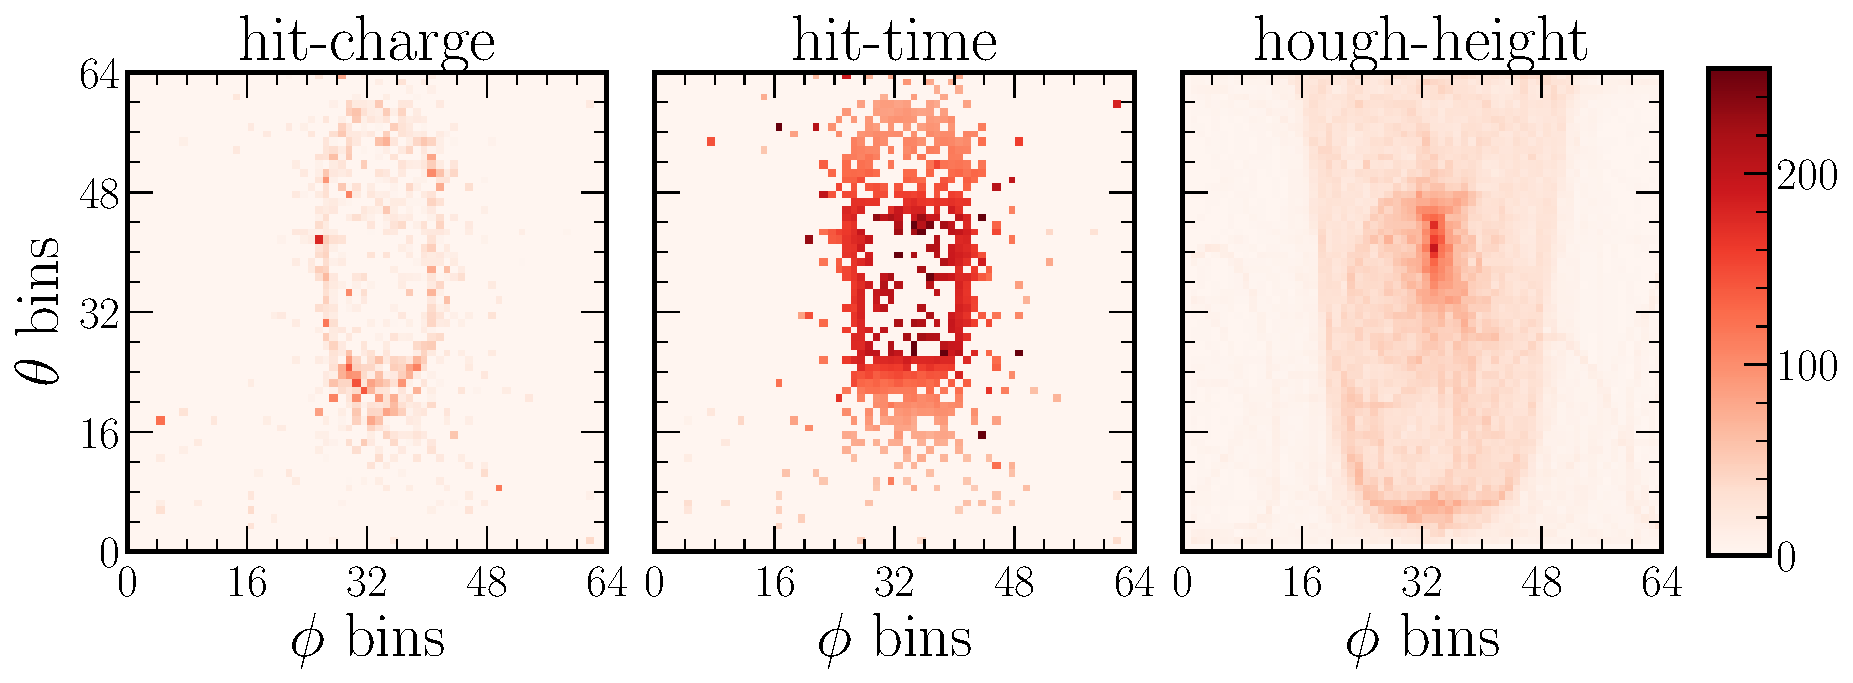
\includegraphics[width=\textwidth]{diagrams/7-results/explore_nuel_ccres_event.pdf}
    \caption[Example of a CC resonant $\nu_{e}$ event]
    {Three map representation of a CC resonant $\nu_{e}$ event. Initiated by a $\nu_{e}$ of energy
        \SI{3.3}{\GeV} the final state particles above the Cherenkov threshold include a $e^{-}$
        of energy \SI{2.8}{\GeV} and a \SI{0.3}{\GeV} $\pi^{0}$.}
    \label{fig:explore_nuel_ccres_event}
\end{figure}

\begin{figure} % NUMU EVENT DIAGRAM %
    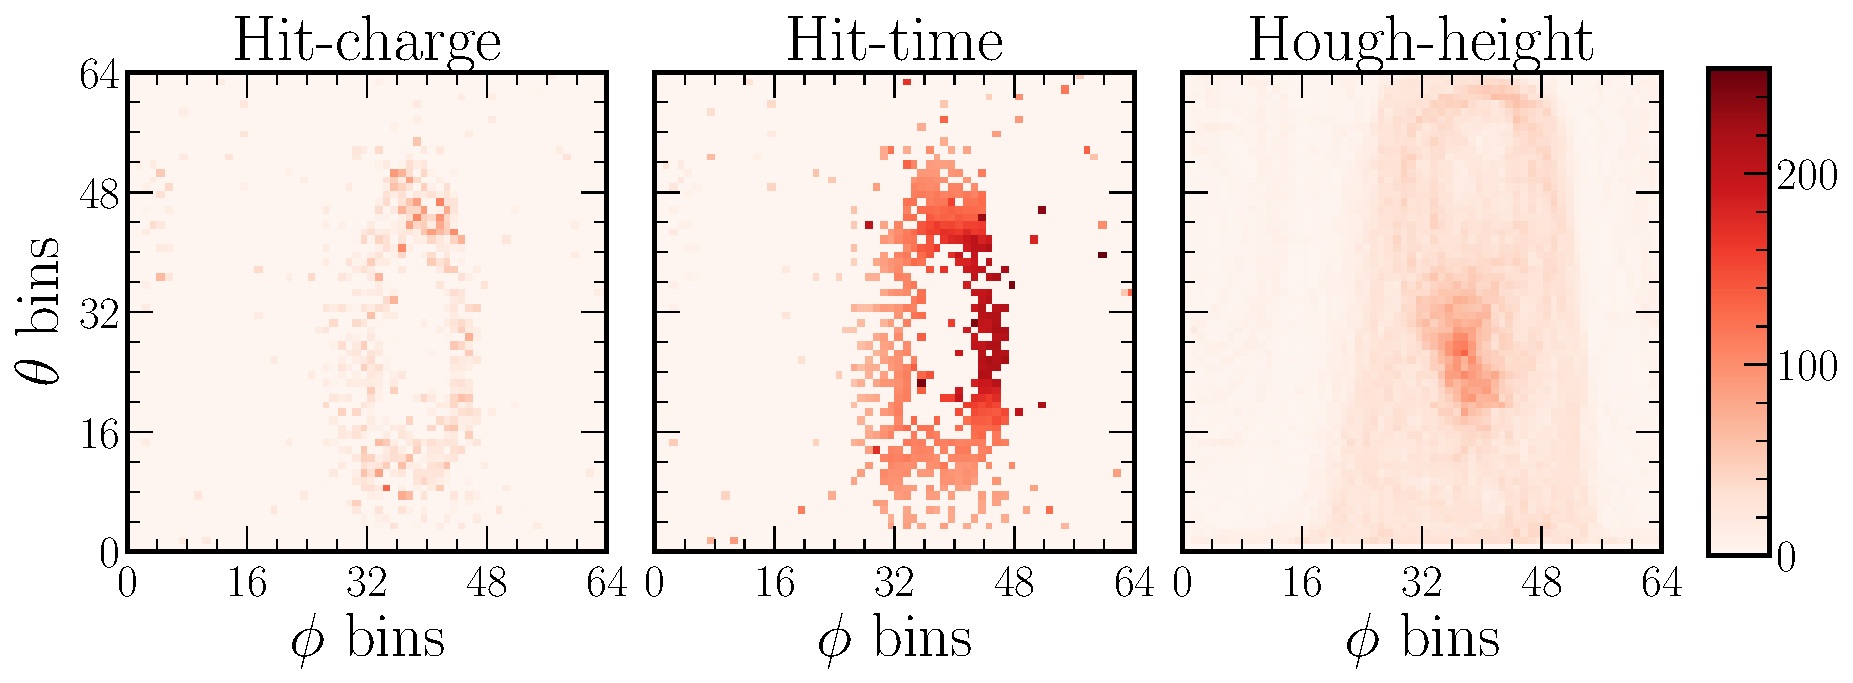
\includegraphics[width=\textwidth]{diagrams/7-results/explore_numu_ccdis_event.pdf}
    \caption[Example of a CC DIS $\nu_{\mu}$ event]
    {Three map representation of a CC DIS $\nu_{\mu}$ event. Initiated by a $\nu_{\mu}$ of energy
        \SI{3.5}{\GeV} the final state particles above the Cherenkov threshold include a $\mu^{-}$
        of energy \SI{1.9}{\GeV}, a proton of energy\SI{2.0}{\GeV}, and a \SI{0.2}{\GeV}
        $\pi^{-}$.}
    \label{fig:explore_numu_ccdis_event}
\end{figure}

\begin{figure} % NC EVENT DIAGRAM %
    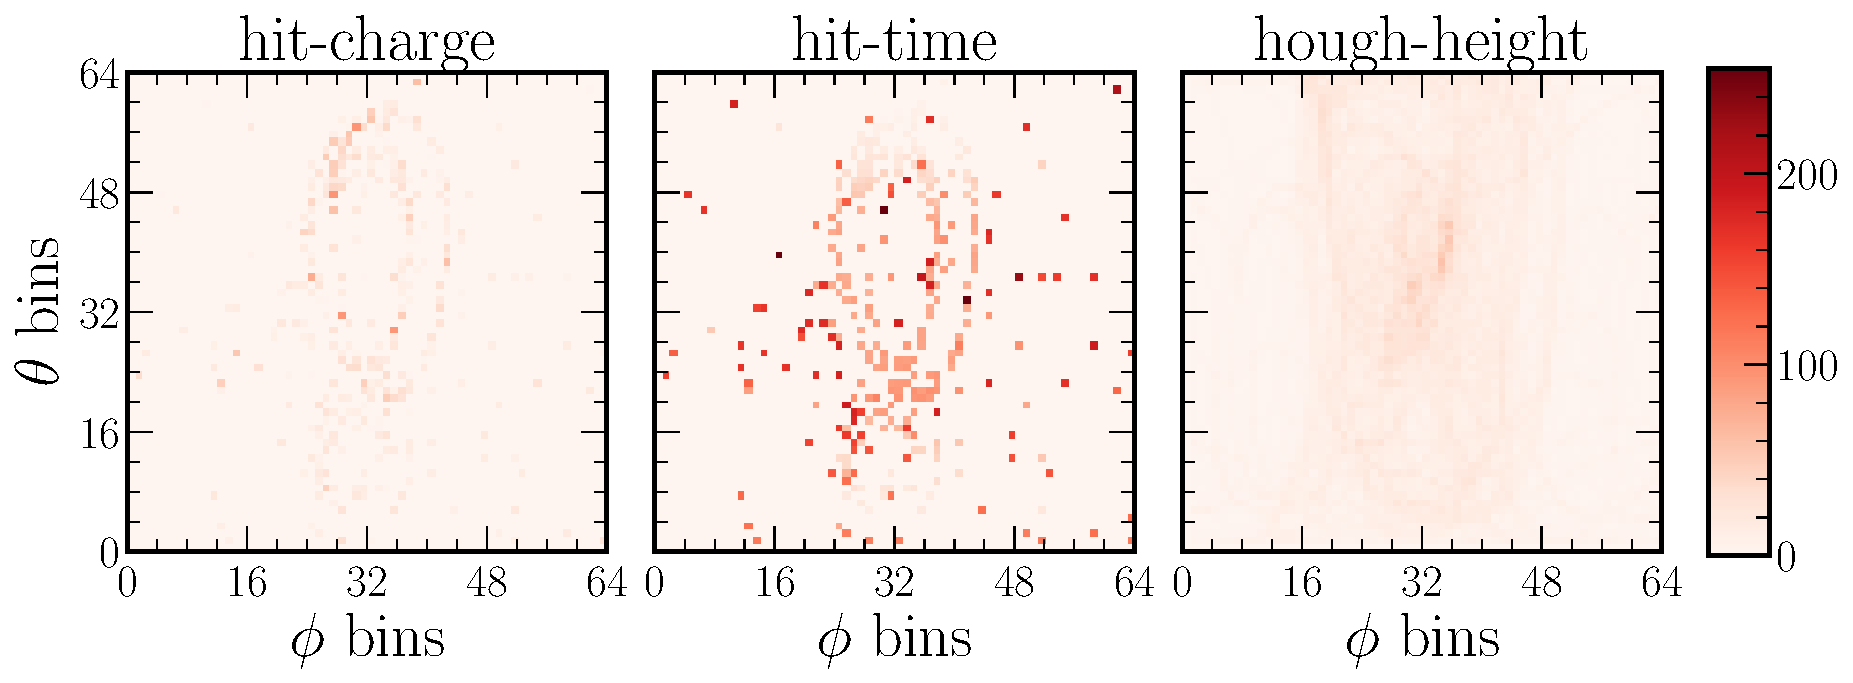
\includegraphics[width=\textwidth]{diagrams/7-results/explore_nuel_ncdis_event.pdf}
    \caption[Example of a NC DIS event]
    {Three map representation of a NC DIS event. Initiated by a $\nu_{e}$ of energy \SI{9.3}{GeV}
        the final state particles above the Cherenkov threshold include a proton of energy
        \SI{2.6}{\GeV} and a \SI{2.5}{\GeV} $\pi^{-}$.}
    \label{fig:explore_nuel_ncdis_event}
\end{figure}

\begin{figure} % COSMIC MUON EVENT DIAGRAM %
    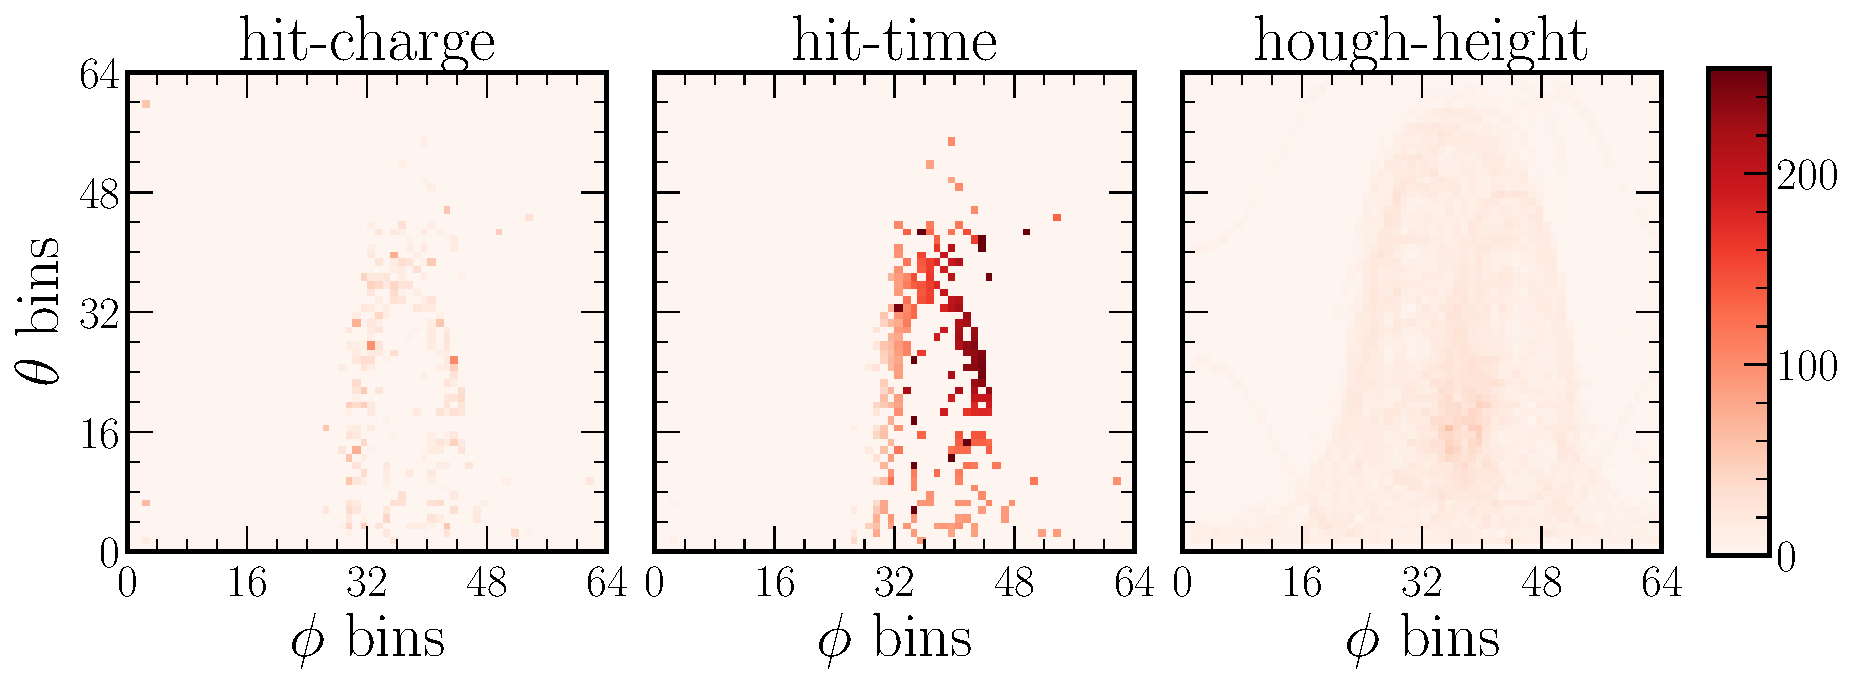
\includegraphics[width=\textwidth]{diagrams/7-results/explore_cosmic_event.pdf}
    \caption[Example of a cosmic muon event]
    {Three channel representation of a cosmic muon event, containing a $\mu^{-}$ of energy
        \SI{2.9}{\GeV}.}
    \label{fig:explore_cosmic_event}
\end{figure}

\subsection{Baseline architecture} %%%%%%%%%%%%%%%%%%%%%%%%%%%%%%%%%%%%%%%%%%%%%%%%%%%%%%%%%%%%%%%
\label{sec:cnn_baseline_arch} %%%%%%%%%%%%%%%%%%%%%%%%%%%%%%%%%%%%%%%%%%%%%%%%%%%%%%%%%%%%%%%%%%%%

An illustrative diagram of the baseline chipsnet architecture is shown in
\FigureRef{fig:chipsnet}. Based on the VGG network previously mentioned in
\SectionRef{sec:cnn_previous} and detailed in \ReferenceRef{simonyan2014} there are a few key
differences from the literature defined network:

\begin{figure} % CHIPSNET DIAGRAM %
    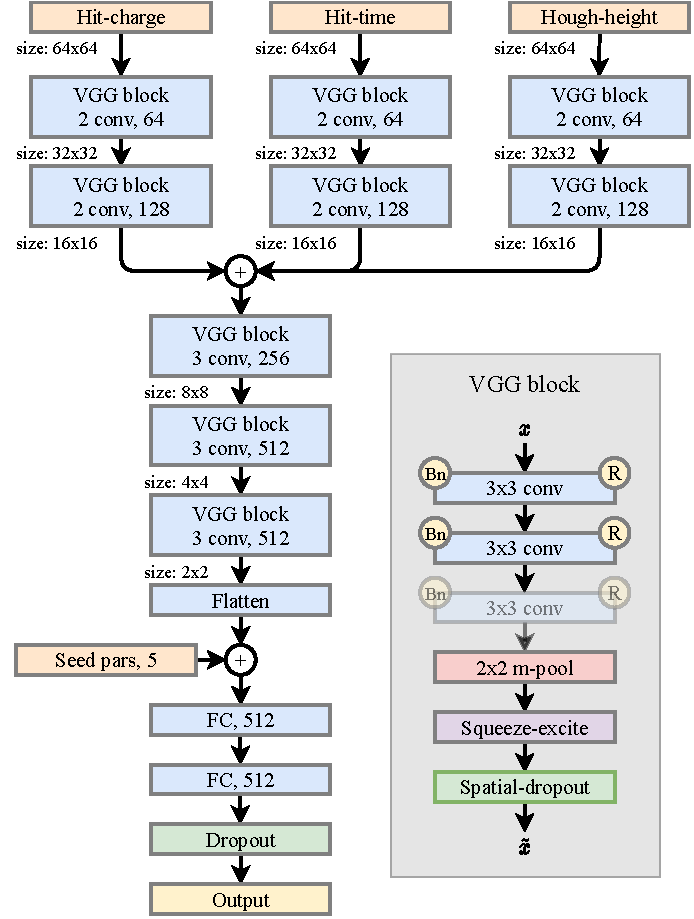
\includegraphics[width=0.7\textwidth]{diagrams/6-cnn/chipsnet.pdf}
    \caption[Illustrative diagram of the baseline chipsnet architecture]
    {Illustrative diagram of the baseline chipsnet architecture. The three input event maps are
        separately passed through two VGG blocks each before their outputs are combined and passed
        through a further three VGG blocks together. The flattened VGG blocks outputs are then
        concatenated with five seed parameters (seed pars) and passed through two fully-connected
        (FC) layers of 512 neurons each before the output layer. Both the number of convolutional
        units (1st value) and kernels (2nd value) is shown for each block. The detailed VGG block
        structure is shown within the grey box. The circular yellow $R$ and $Bn$ indicate the use
        of the ReLU activation function and batch normalisation, respectively.}
    \label{fig:chipsnet}
\end{figure}

\begin{itemize}
    \item Each of the three event maps: hit-charge, hit-time, and hough-height are initially fed
          into three separate branches. Each branch contains two VGG blocks with two convolutional
          layers each (four convolutional layers in total). The outputs from each branch are
          merged using a concatenation layer before being fed to the rest of the network. This
          configuration allows for event map specific features to be learnt independently before
          combined features are learnt by the rest of the network.

    \item Batch normalisation as described in \SectionRef{sec:cnn_theory_reg} is included before
          the activation (ReLU) function for every convolutional layer.

    \item Squeeze-and-excitation units, as detailed in \ReferenceRef{hu2018} are included after
          the max-pooling operation in all VGG blocks. These units introduce extra parameters to
          model the interdependencies between output feature maps, allowing the network to learn
          how to weight each feature map effectively.

    \item Dropout is included at the end of each VGG block as well as after the final
          fully-connected layer. Instead of dropping individual kernel elements, the dropout
          within the VGG blocks drops entire kernels at each training iteration, this is commonly
          called \emph{two-dimensional spatial dropout}. The dropout after the fully-connected
          layers is standard, in that it drops out individual fully-connected neurons.

    \item Five output parameters from the seeding process (seed pars) are concatenated with the
          flattened layer before the fully-connected layers. Included are the three components of
          the estimated interaction vertex position ($s_{x},s_{y}, s_{z}$), and the two components
          of the estimated track direction ($s_{\theta},s_{\phi}$). These parameters provide the
          network with spatial context as to where in the detector the input event maps have been
          generated and the dominant direction of PMT activity.
\end{itemize}

The chipsnet baseline architecture is implemented using the Keras API built into
Tensorflow~\cite{chollet2015}. Keras allows for predefined common layers such as a two-dimensional
convolution or a max-pooling layer to be easily structured into a full network definition.

\subsection{Baseline outputs} %%%%%%%%%%%%%%%%%%%%%%%%%%%%%%%%%%%%%%%%%%%%%%%%%%%%%%%%%%%%%%%%%%%%
\label{sec:cnn_baseline_outputs} %%%%%%%%%%%%%%%%%%%%%%%%%%%%%%%%%%%%%%%%%%%%%%%%%%%%%%%%%%%%%%%%%

Many CNN applications are found to benefit from learning multiple tasks at the same time. This is
believed to be the case as training with multiple tasks tends to return a network with an improved
generalised representation of the inputs, with features learnt for one task improving the
performance of another. Additionally, multiple tasks work to prevent any one output from
overfitting. Commonly named \emph{multi-task} learning, this methodology is used extensively in
this work.

To train a network with multiple tasks (outputs), a loss function $E_{tot}$, must be defined to
combine the individual loss functions for each task $E_{i}$. The simplest way to do this is via a
linear weighted sum, such that
\begin{equation}
    E_{tot} = \sum_{i=1}^{i=N}w_{i}E_{i},
    \label{eq:multi_simple}
\end{equation}
where $N$ is the number of tasks and $w_{i}$ are the associated weights. In this work this is
referred to as the \emph{simple} multi-task loss.

However, the final network performance can strongly depend on the relative weighting between loss
functions, especially when the values returned by each differ by many order of magnitude (common
when combining regression and classification tasks). Therefore, finding the optimal $w_{i}$
weights can be both difficult and time-consuming. Another approach outlined in
\ReferenceRef{kendall2018} remedies this problem by learning the optimal weighting between loss
functions. This is done by introducing an additional trainable parameter $\sigma_{i}$, for each
loss function, such that
\begin{equation}
    E_{tot}= \sum_{i=1}^{i=N}\frac{1}{2\sigma_{i}^2}E_{i}+ \log\sigma_{i}.
    \label{eq:multi_learnt}
\end{equation}
In this work we refer to this as the \emph{learnt} multi-task loss.

The specific number and nature of outputs for the specific networks are detailed in
\SectionRef{sec:cnn_specific}. Although physically motivated to some degree, the exact set of
tasks and the loss combination technique used is mainly driven by extensive trial-and-error. The
chipsnet software is specifically designed to enable this process by making it easy to configure
the network outputs via a simple configuration file.

\subsection{Baseline training} %%%%%%%%%%%%%%%%%%%%%%%%%%%%%%%%%%%%%%%%%%%%%%%%%%%%%%%%%%%%%%%%%%%
\label{sec:cnn_baseline_training} %%%%%%%%%%%%%%%%%%%%%%%%%%%%%%%%%%%%%%%%%%%%%%%%%%%%%%%%%%%%%%%%

All networks are trained on an 18 core CPU (36 thread) machine equipped with four NVIDIA GeForce
RTX 2080 graphics processing units (GPUs). The Tensorflow dataset API is used to create an
efficient input data pipeline where data is loaded on-the-fly at training time. This procedure
ensures all CPU threads are utilised loading, decoding, and preprocessing data for the primary GPU
based network calculations before being needed, maximising computational efficiency.

During preprocessing, all 8-bit input event map values are converted to 32-bit float values
bounded between zero and one. Furthermore, a random factor scaling is applied to each map bin.
Generated from a normal distribution centred on one with a standard deviation of $\sigma_{r}$, by
fluctuating the bin values the network is forced to focus less on the absolute bin values and more
on the underlying event topology. Not only does this process provide valuable regularisation to
reduce overfitting, but also makes the trained networks robust to small changes within the input
(explored within \SectionRef{sec:results_robust}).

A minibatch training strategy of minibatch size of $n_{b}$, using the Adam
optimiser~\cite{kingma2014} ($\beta_{1}=0.9$, $\beta_{2}=0.999$, and $\epsilon = 1e-7$) is used.
The exact training sample size and composition for each specific network are given in
\SectionRef{sec:cnn_specific}, but for all networks a 95\% training to 5\% validation data split
is employed across the full training sample. Consequently, early stopping is used. The learning
rate for each epoch $\eta_{e}$, is set to decrease throughout training according to
\begin{equation}
    \eta_{e}=\frac{\eta_{0}}{1+c_{d}(e-1)},
\end{equation}
where $\eta_{0}$ is the initial learning rate, $e$ is the epoch number (starting at one), and
$c_{d}$ is the learning rate decay coefficient.

Therefore, when training each network, there is a list of tunable \emph{hyperparameters}, all of
which are optimised using the SHERPA hyperparameter tuning framework~\cite{hertel2020}. To
maximise performance, SHERPA uses a \emph{random search} algorithm to select random configurations
of hyperparameters which are then tested by training the network for five epochs on the available
training data. Each configuration's performance is assessed by using a metric detailed for each
network in \SectionRef{sec:cnn_specific}. The search space is confined to a specific range or
selection of choices for each hyperparameter, with:
\begin{itemize}
    \item the \textbf{initial learning rate $\eta_{0}$}, in a range from $0.00005$ to $0.001$;
    \item the \textbf{learning rate decay coefficient $c_{d}$}, in a range from $0.2$ to $0.8$;
    \item the \textbf{dropout probability $p_{d}$}, in a range from $0.0$ to $0.5$;
    \item the \textbf{random scaling size $\sigma_{r}$}, in a range from $0.0$ to $0.1$;
    \item the \textbf{minibatch size $n_{b}$}, choosing from either $32$, $64$, $128$, or $256$;
    and
    \item the \textbf{multi-task loss combination strategy}, choosing from either simple or
    learnt.
\end{itemize}

\section{Specific implementations for CHIPS} %%%%%%%%%%%%%%%%%%%%%%%%%%%%%%%%%%%%%%%%%%%%%%%%%%%%%
\label{sec:cnn_specific} %%%%%%%%%%%%%%%%%%%%%%%%%%%%%%%%%%%%%%%%%%%%%%%%%%%%%%%%%%%%%%%%%%%%%%%%%

The specific CNN implementations for cosmic rejection, beam classification, and energy estimation
are outlined below. It is important to note that the exact configuration of networks outlined here
is the result of extensive testing designed to maximise the selection of a pure and efficient
sample of appeared CC $\nu_{e}$ beam events whose neutrino energy can also be accurately
determined.

As an example of an alternative implementation, if cosmic rejection and beam classification are
combined into a single network, both objectives see a reduction in performance. The same is also
true if either cosmic rejection or beam classification is combined with neutrino energy
estimation. However, specific secondary outputs such as counting the number of primary particles
in conjunction with beam classification are seen to improve performance. It is clear, therefore,
that the multi-task approach only works for tasks that require a similar learnt representation of
the inputs. Put simply; the tasks must be similar.

\subsection{Cosmic rejection} %%%%%%%%%%%%%%%%%%%%%%%%%%%%%%%%%%%%%%%%%%%%%%%%%%%%%%%%%%%%%%%%%%%%
\label{sec:cnn_specific_cosmic} %%%%%%%%%%%%%%%%%%%%%%%%%%%%%%%%%%%%%%%%%%%%%%%%%%%%%%%%%%%%%%%%%%

The cosmic rejection network aims to prevent the vast cosmic muon background from contaminating
the final selected sample of beam events. Therefore, the primary task is a simple binary
classification between beam and cosmic events. Additionally, training the network to also separate
events where the primary charged lepton escapes the detector volume or not, is found to improve
cosmic rejection performance. As a large proportion of cosmic muons are relatively high in energy
and, therefore, escape the detector in this fashion, there is motivation as to why this additional
task is helpful.

The network is trained on a sample of 3.15 million simulated events produced using the detector
simulation and event generation methods outlined in \SectionRef{sec:chips_monte_carlo}. Roughly
$1/3^{rd}$ are $\nu_{\mu}$ beam events, $1/3^{rd}$ $\nu_{e}$ beam events, and $1/3^{rd}$ cosmic
muon events, the counts of which are shown in \FigureRef{fig:cosmic_training_sample}. All beam
events (both $\nu_{\mu}$ and $\nu_{e}$) are generated using the expected unoscillated \chipsfive
$\nu_{\mu}$ energy spectrum to closely mimic the dominant $\nu_{\mu}$ beam component and appeared
$\nu_{e}$ signal. Every event in the sample is used for training with no preselection, as this is
found to be the best for cosmic rejection performance.

\begin{figure} % COSMIC TRAINING SAMPLE DIAGRAM %
    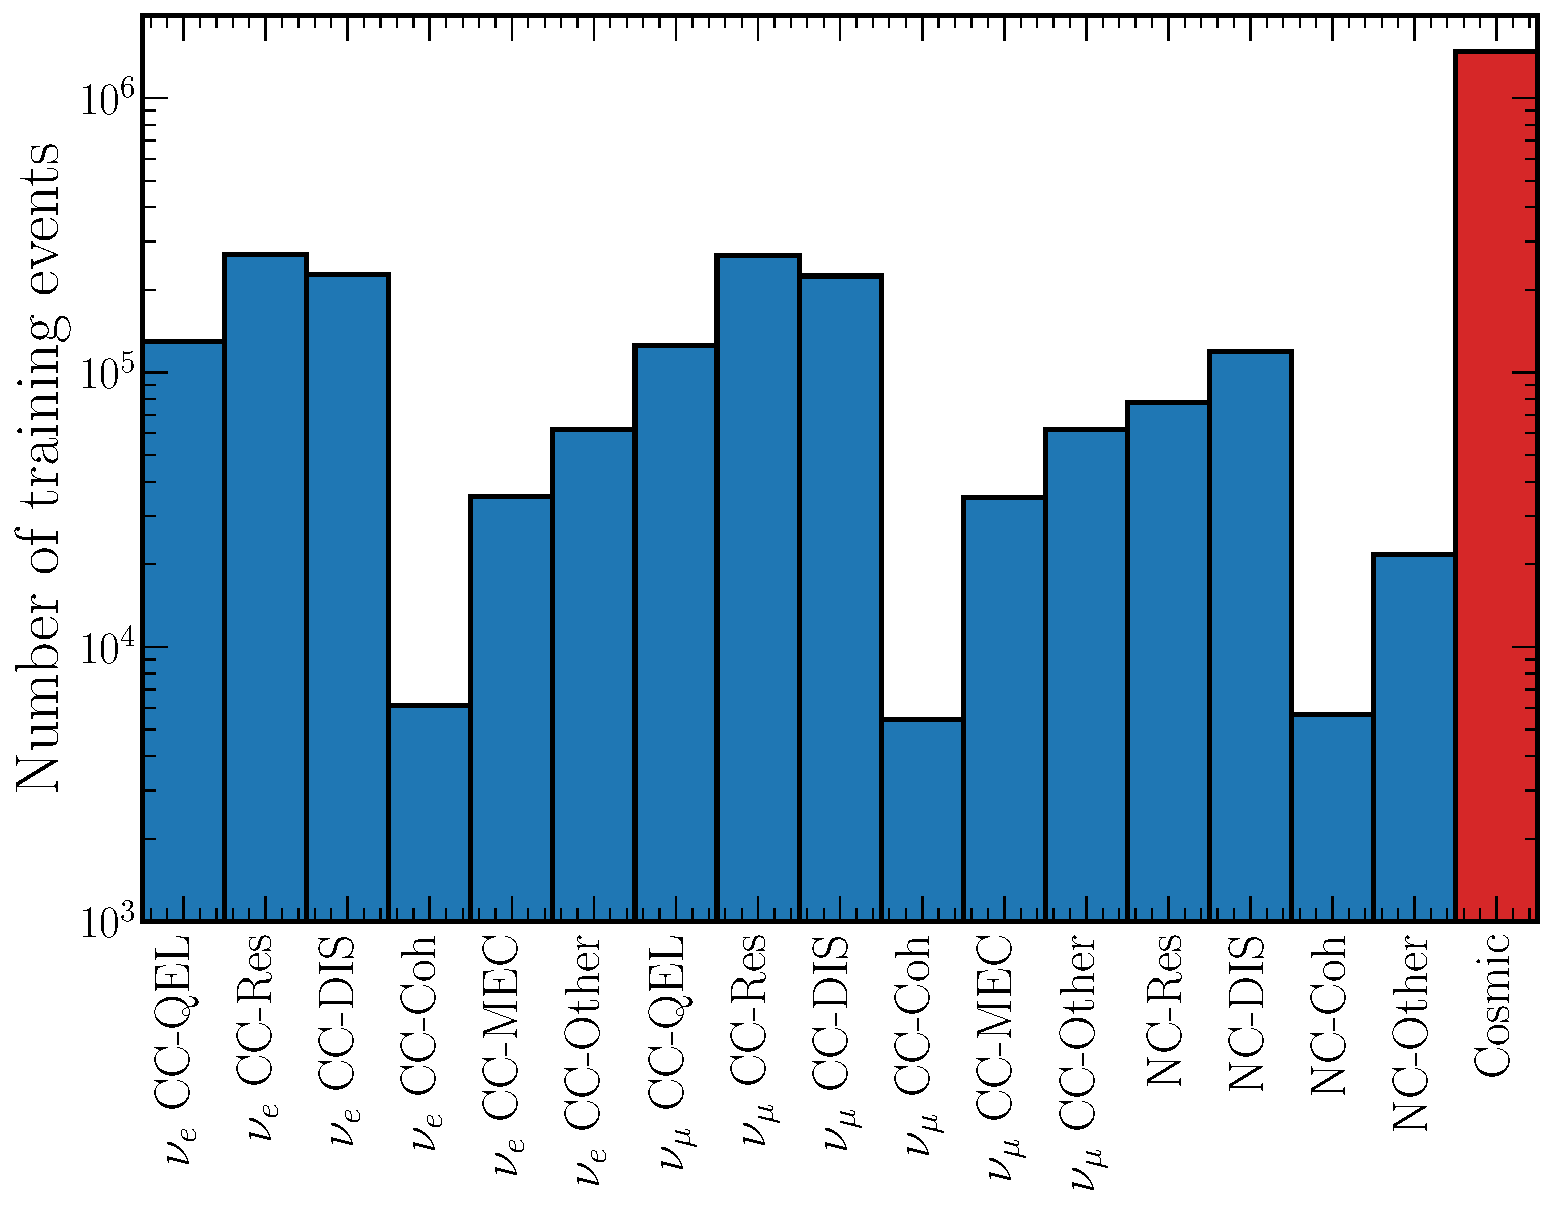
\includegraphics[width=0.7\textwidth]{diagrams/7-results/explore_cosmic_training_sample.pdf}
    \caption[Number of training events per category for the cosmic rejection network]
    {Number of training events per category for the cosmic rejection network. All beam event
        interaction types are shown, however, all are classed as beam events (blue) in training
        against the cosmic events (red).}
    \label{fig:cosmic_training_sample}
\end{figure}

There are two outputs to the cosmic rejection network:
\begin{enumerate}
    \item \textbf{Cosmic score (1 classification neuron):} Returns a score between zero and one
          corresponding to whether the event is beam or cosmic like. The binary cross-entropy loss
          function in \EquationRef{eq:binary_cross_entropy} is used for training with a simple
          multi-task weight of $1$.
    \item \textbf{Escapes score (1 classification neuron):} Returns a score between zero and one
          corresponding to whether the charged lepton in an event is contained or escapes the
          detector. The binary cross-entropy loss function in
          \EquationRef{eq:binary_cross_entropy} is used for training with a simple multi-task
          weight of $1$. NC beam events without a charged lepton are masked (do not contribute to
          the loss) during training for this output.
\end{enumerate}

The network is allowed to train for up to 30 epochs using the SHERPA optimised hyperparameters:
$\eta_{0}=0.00005$, $c_{d}=0.7$, $p_{d}=0.1$, $\sigma_{r}=0.02$, and $n_{b}=128$, with a simple
multi-task loss combination as given in \EquationRef{eq:multi_simple}. The \emph{cosmic score}
accuracy metric is used for SHERPA optimisation and early stopping, defined as the fraction of
validation sample events that are correctly classified when a cut value of 0.5 on the \emph{cosmic
score} output is used to determine the classification of each event. Typically, only 6 epochs are
required to reach the maximum validation sample \emph{cosmic score} accuracy, with early stopping
halting training after 11 epochs (taking 15 hours), as can be seen in
\FigureRef{fig:final_cosmic_history}.

\begin{figure} % COSMIC HISTORY DIAGRAM %
    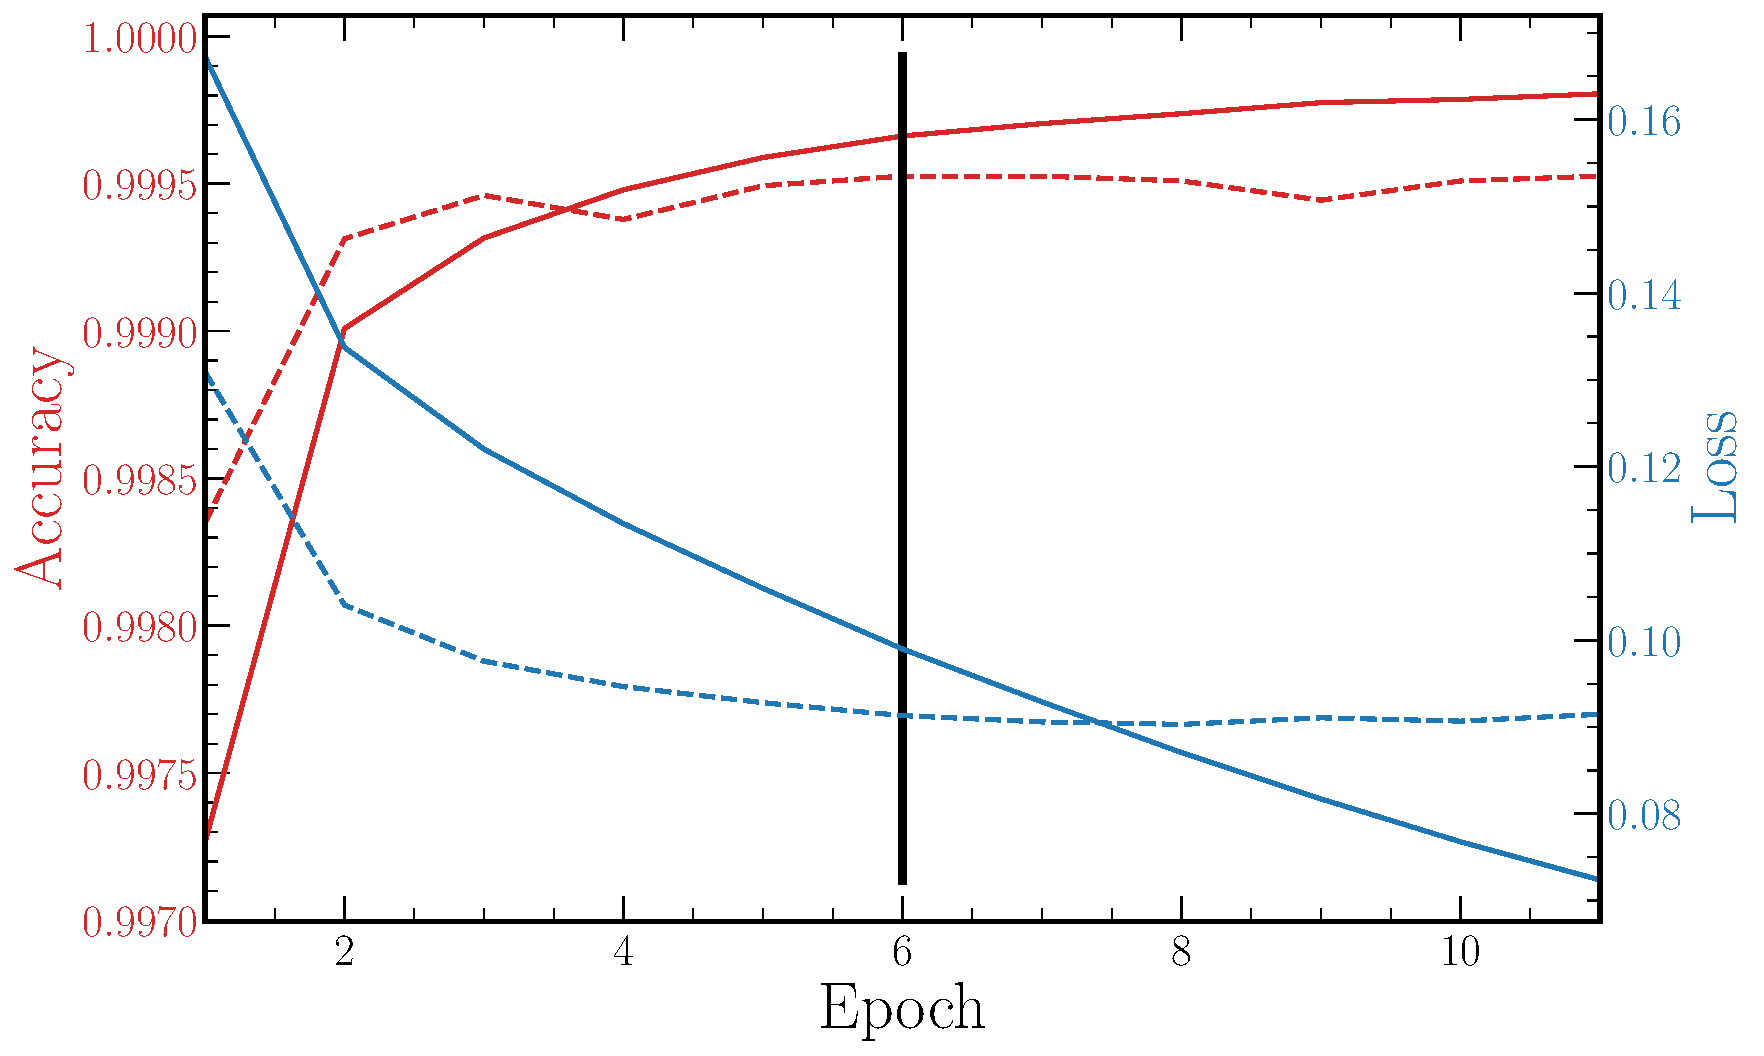
\includegraphics[width=0.7\textwidth]{diagrams/7-results/final_cosmic_history.pdf}
    \caption[Loss and accuracy throughout training for the cosmic rejection network]
    {Total loss and \emph{cosmic score} accuracy for both the training sample (solid) and
        validation sample (dashed) throughout training for the cosmic rejection network. The final
        network weights are taken at epoch six, as shown by the vertical black line.}
    \label{fig:final_cosmic_history}
\end{figure}

\subsection{Beam classification}%%%%%%%%%%%%%%%%%%%%%%%%%%%%%%%%%%%%%%%%%%%%%%%%%%%%%%%%%%%%%%%%%%
\label{sec:cnn_specific_beam} %%%%%%%%%%%%%%%%%%%%%%%%%%%%%%%%%%%%%%%%%%%%%%%%%%%%%%%%%%%%%%%%%%%%

The beam classification network aims to separate beam events by their neutrino and interaction
type to primarily select a pure and efficient sample of appeared $\nu_{e}$ events, but also a
sample of survived CC $\nu_{\mu}$ events. Therefore, the principal task is a categorical
classification between CC $\nu_{e}$, CC $\nu_{\mu}$, and NC events. No attempt is made to separate
the appeared CC $\nu_{e}$ and intrinsic beam CC $\nu_{e}$ components as they are impossible to
tell apart, except for their distribution in neutrino energy.

Similar to the implementation used by DUNE~\cite{collaboration2020}, alongside the core
classification additional classification and particle counting tasks outlined below are included
to improve performance. Note that the particle counting tasks are not used in this work for
anything but increasing the primary classification performance. Future work, however, could
exploit any ability to separate exclusive final states, deduced from these particle counts, to
reduce both energy resolution and systematic errors. As an example of a method already in use,
\nova use their ability to accurately determine the hadronic energy of an event to split their CC
$\nu_{\mu}$ sample into populations of different energy resolution. Each population can then be
treated separately in the analysis before being combined, increasing overall
performance~\cite{acero2018}.

The network is trained on a sample of 1.67 million simulated events produced using the detector
simulation and event generation methods outlined in \SectionRef{sec:chips_monte_carlo}. Roughly
half are $\nu_{\mu}$ beam events, with the other half being $\nu_{e}$ beam events, as shown in
\FigureRef{fig:beam_training_sample}. All events (both $\nu_{\mu}$ and $\nu_{e}$) are generated
using the expected unoscillated \chipsfive $\nu_{\mu}$ energy spectrum to closely mimic the
dominant $\nu_{\mu}$ beam component and appeared $\nu_{e}$ signal. All events are used for
training with no preselection as this is found to be the best for beam classification performance,
especially NC rejection.

\begin{figure} % BEAM TRAINING SAMPLE DIAGRAM %
    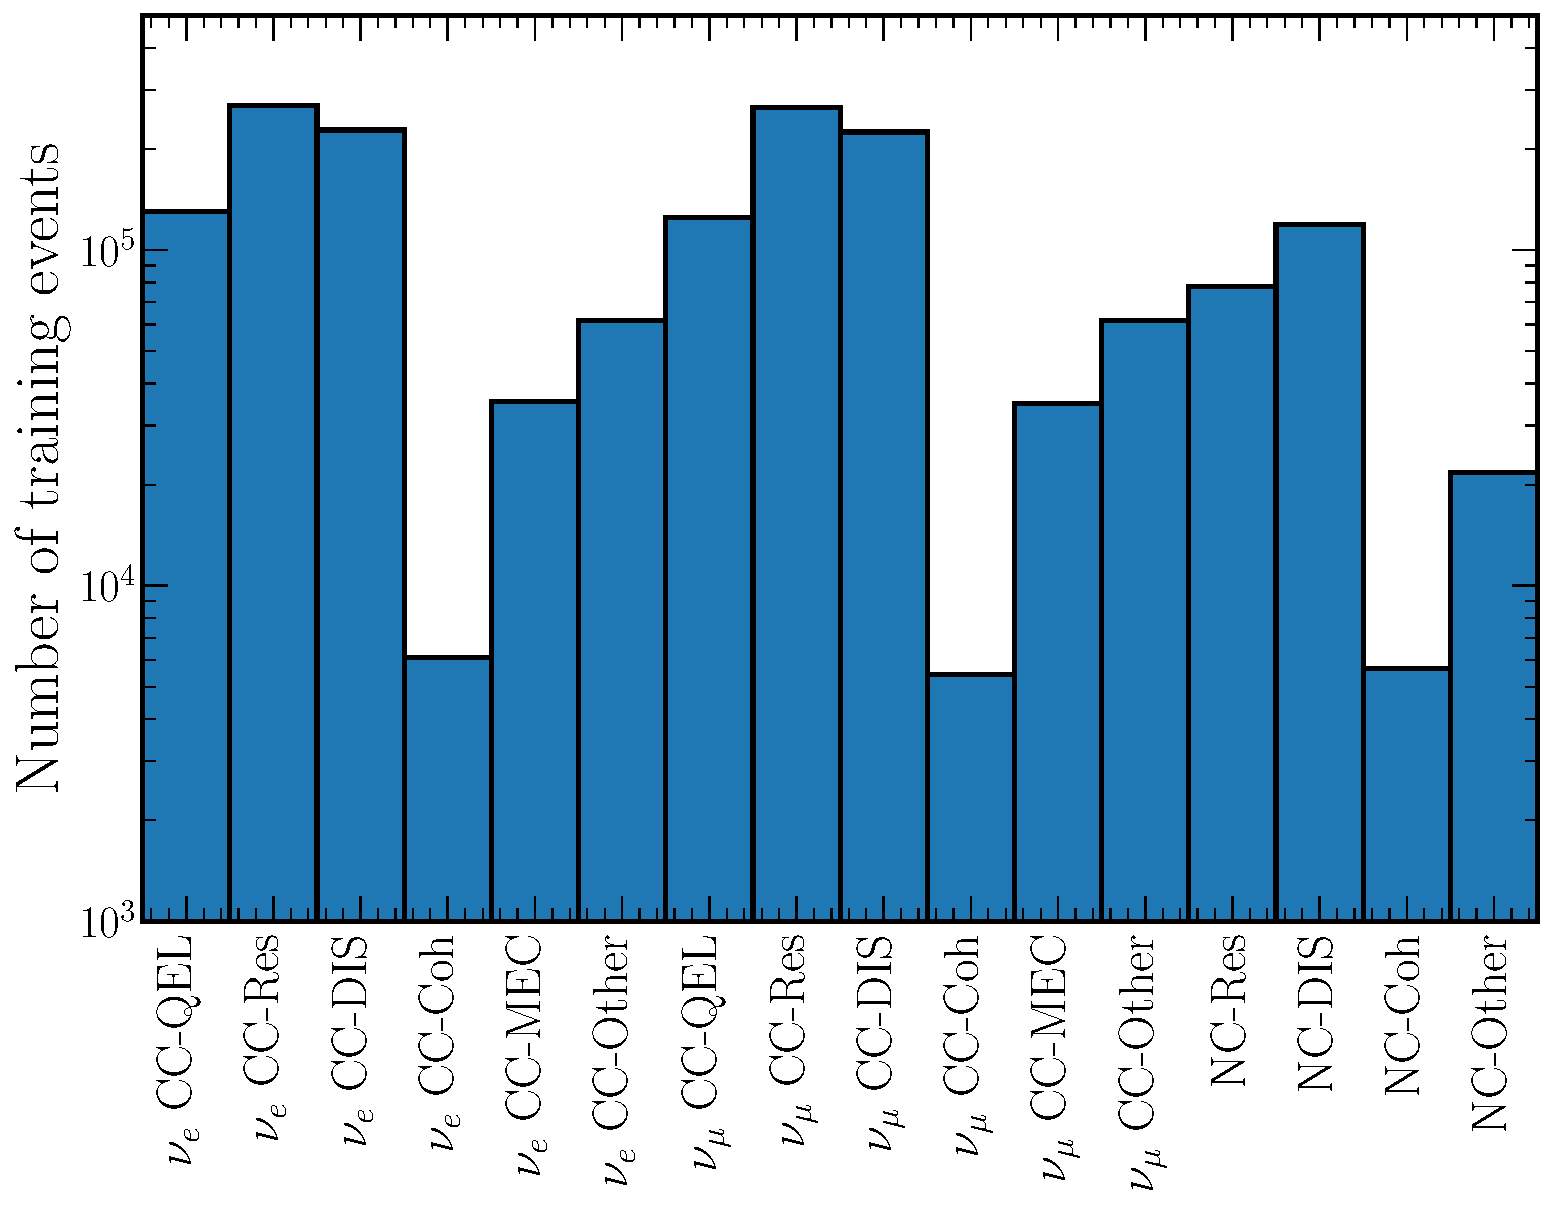
\includegraphics[width=0.7\textwidth]{diagrams/7-results/explore_beam_training_sample.pdf}
    \caption[Number of training events per category for the beam classification network]
    {Number of training events per category for the beam classification network. All beam event
        interaction types are shown.}
    \label{fig:beam_training_sample}
\end{figure}

There are nine outputs to the beam classification network:
\begin{enumerate}
    \item \textbf{Combined category (3 classification neurons):} Returns a classification
          probability score between zero and one for each of CC $\nu_{e}$, CC $\nu_{\mu}$, and NC
          (summing to one). The categorical cross-entropy loss function in
          \EquationRef{eq:categorical_cross_entropy} is used for training with a simple multi-task
          weight of $1$.
    \item \textbf{CC category (6 classification neurons):} Returns a classification probability
          score between zero and one for each of CC-QEL, CC-Res, CC-DIS, CC-Coh, CC-MEC, and
          CC-other (summing to one). The categorical cross-entropy loss function in
          \EquationRef{eq:categorical_cross_entropy} is used for training with a simple multi-task
          weight of $1$. NC events are masked (do not contribute to the loss) during training for
          this output.
    \item \textbf{NC category (4 classification neurons):} Returns a classification probability
          score between zero and one for each of NC-Res, NC-DIS, NC-Coh, and NC-other (summing to
          one). The categorical cross-entropy loss function in
          \EquationRef{eq:categorical_cross_entropy} is used for training with a simple multi-task
          weight of $1$. CC events are masked (do not contribute to the loss) during training for
          this output.
    \item \textbf{Electron count (4 classification neurons):} Returns a classification probability
          score between zero and one for each of 0, 1, 2, and 3+ electrons in the final state
          (summing to one). The categorical cross-entropy loss function in
          \EquationRef{eq:categorical_cross_entropy} is used for training with a simple multi-task
          weight of $1$.
    \item \textbf{Muon count (4 classification neurons):} Returns a classification probability
          score between zero and one for each of 0, 1, 2, and 3+ muons in the final state (summing
          to one). The categorical cross-entropy loss function in
          \EquationRef{eq:categorical_cross_entropy} is used for training with a simple multi-task
          weight of $1$.
    \item \textbf{Proton count (4 classification neurons):} Returns a classification probability
          score between zero and one for each of 0, 1, 2, and 3+ protons in the final state
          (summing to one). The categorical cross-entropy loss function in
          \EquationRef{eq:categorical_cross_entropy} is used for training with a simple multi-task
          weight of $1$.
    \item \textbf{$\pi^{\pm}$ count (4 classification neurons):} Returns a classification
          probability score between zero and one for each of 0, 1, 2, and 3+ charged pions in the
          final state (summing to one). The categorical cross-entropy loss function in
          \EquationRef{eq:categorical_cross_entropy} is used for training with a simple multi-task
          weight of $1$.
    \item \textbf{$\pi^{0}$ count (4 classification neurons):} Returns a classification
          probability score between zero and one for each of 0, 1, 2, and 3+ neutral pions in the
          final state (summing to one). The categorical cross-entropy loss function in
          \EquationRef{eq:categorical_cross_entropy} is used for training with a simple multi-task
          weight of $1$.
    \item \textbf{Photon count (4 classification neurons):} Returns a classification probability
          score between zero and one for each of 0, 1, 2, and 3+ photons in the final state
          (summing to one). The categorical cross-entropy loss function in
          \EquationRef{eq:categorical_cross_entropy} is used for training with a simple multi-task
          weight of $1$.
\end{enumerate}

The network is allowed to train for up to 30 epochs using the SHERPA optimised hyperparameters:
$\eta_{0}=0.0002$, $c_{d}=0.5$, $p_{d}=0.1$, $\sigma_{r}=0.02$, and $n_{b}=128$, with a simple
multi-task loss combination as given in \EquationRef{eq:multi_simple}. The \emph{combined
category} accuracy metric is used for SHERPA optimisation and early stopping, defined as the
fraction of validation sample events that are correctly classified when the highest scoring
\emph{combined category} output neuron is used to determine the classification of each event.
Typically, only 7 epochs are required to reach the maximum validation sample \emph{combined
category} accuracy, with early stopping halting training after 12 epochs (taking 15 hours), as can
be seen in \FigureRef{fig:final_beam_history}.

\begin{figure} % BEAM HISTORY DIAGRAM %
    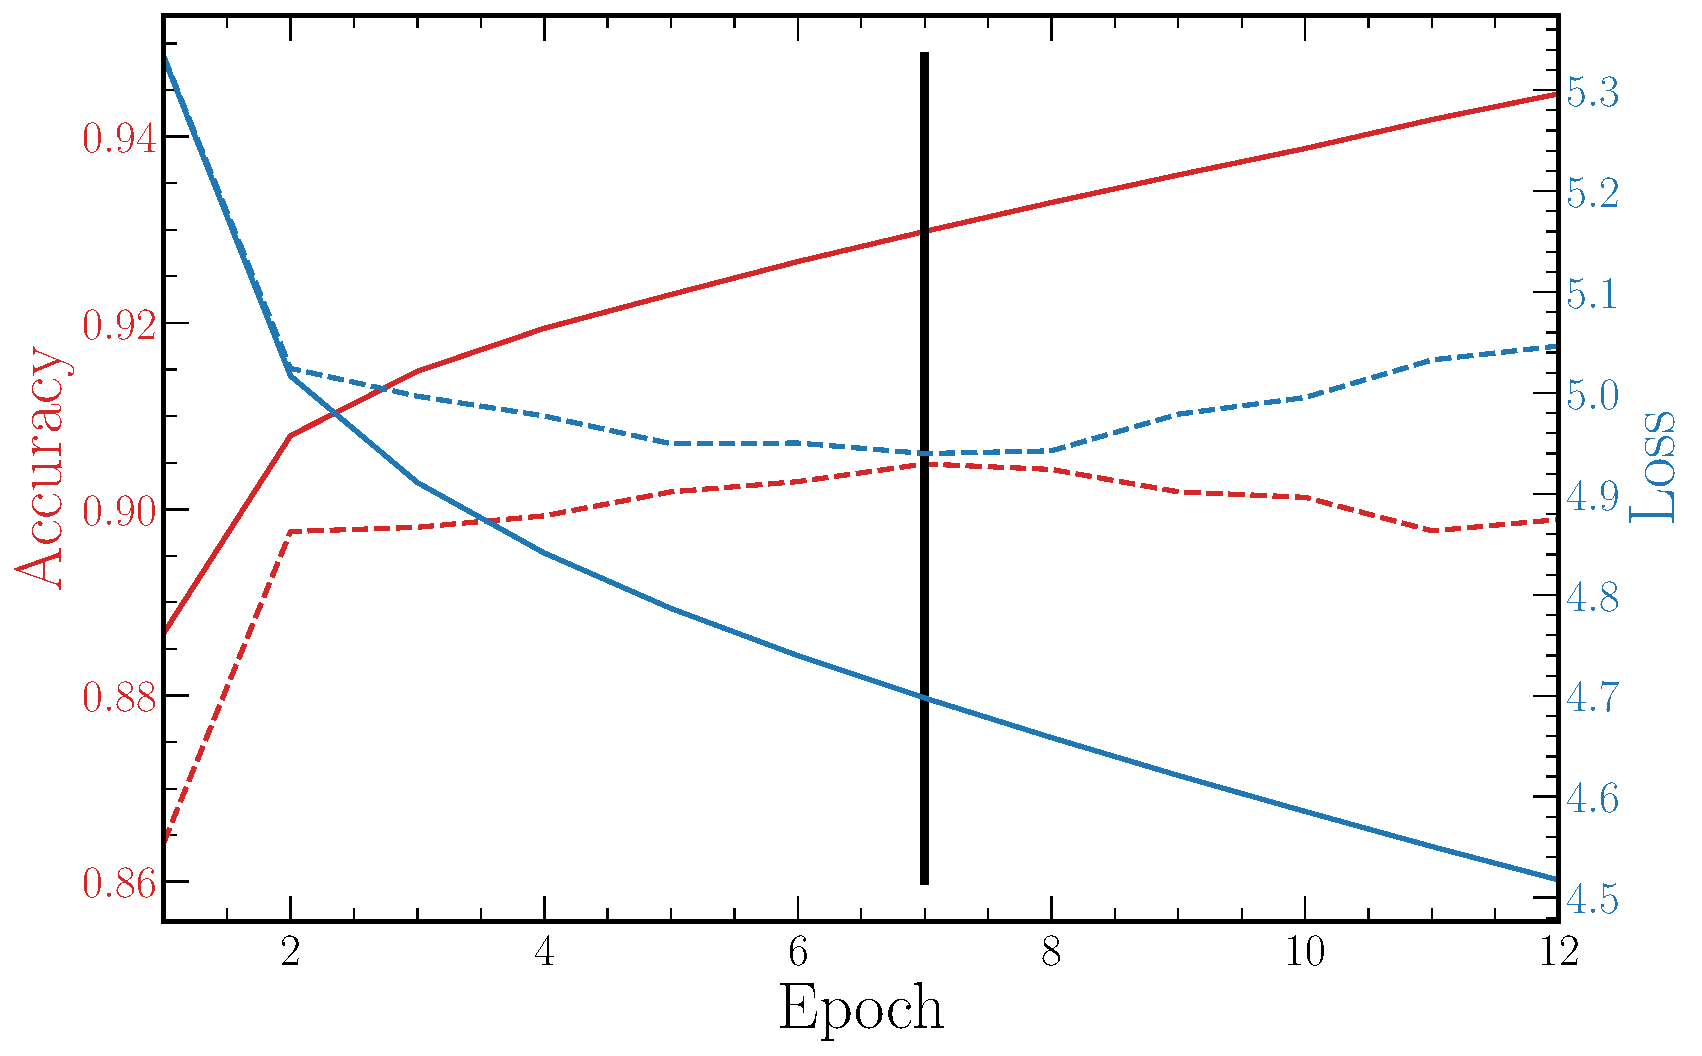
\includegraphics[width=0.7\textwidth]{diagrams/7-results/final_beam_history.pdf}
    \caption[Loss and accuracy throughout training for the beam classification network]
    {Total loss and \emph{combined category} accuracy for both the training sample (solid) and
        validation sample (dashed) throughout training for the beam classification network. The
        final network weights are taken at epoch seven, as shown by the vertical black line.}
    \label{fig:final_beam_history}
\end{figure}

\subsection{Energy estimation} %%%%%%%%%%%%%%%%%%%%%%%%%%%%%%%%%%%%%%%%%%%%%%%%%%%%%%%%%%%%%%%%%%%
\label{sec:cnn_specific_energy} %%%%%%%%%%%%%%%%%%%%%%%%%%%%%%%%%%%%%%%%%%%%%%%%%%%%%%%%%%%%%%%%%%

Accurate neutrino energy estimation is accomplished using multiple networks trained on separate
samples of $\nu_{e}$ and $\nu_{\mu}$ events across multiple CC interaction types. It is found that
separation such as this results in greater performance compared to if a single energy estimation
network or even separate $\nu_{e}$ and $\nu_{\mu}$ networks are trained. This is expected as a
single set of network weights is unlikely to be able to capture the specific topological features
that contribute to the energy for all types of event.

Alongside the primary neutrino energy regression task, additionally learning the primary charged
lepton energy and the interaction vertex position and time are found to improve performance.
Although this improvement is relatively small for neutrino energy estimation, it dramatically
improves primary charged lepton energy estimation when compared to being predicted alone. With two
energy tasks, the network is encouraged to learn how the primary charged lepton and neutrino
energies are related. As the interaction vertex position within the detector and hence distance
from the instrumented wall can impact the number of deposited photoelectrons, there is motivation
as to why this additional task is also helpful.

Separate networks are trained for each of CC-QEL (and CC-MEC), CC-Res, and CC-DIS for both
$\nu_{e}$ and $\nu_{\mu}$ events (6 in total) using 250000 corresponding simulated events each.
All events (both $\nu_{\mu}$ and $\nu_{e}$) are produced using the detector simulation and event
generation methods outlined in \SectionRef{sec:chips_monte_carlo}. The expected unoscillated
\chipsfive $\nu_{\mu}$ energy spectrum is used to generate all events to closely mimic the
dominant $\nu_{\mu}$ beam component and appeared $\nu_{e}$ signal. Only events for which the
primary charged lepton is fully contained within the detector volume are used for training, with
no additional preselection applied. Note that CC-QEL and CC-MEC energy estimation is combined into
a single network as both have incredibly similar final state topologies (a single charged lepton).

There are six outputs to each of the energy estimation networks:
\begin{enumerate}
    \item \textbf{Neutrino energy (1 regression neuron):} Returns the estimated neutrino energy.
          The mean-squared error loss function in \EquationRef{eq:mse} is used for training.
    \item \textbf{Charged lepton energy (1 regression neuron):} Returns the estimated primary
          charged lepton energy. The mean-squared error loss function in \EquationRef{eq:mse} is
          used for training.
    \item \textbf{Interaction vertex x-position (1 regression neuron):} Returns the estimated
          interaction vertex x-position. The mean-squared error loss function in
          \EquationRef{eq:mse} is used for training.
    \item \textbf{Interaction vertex y-position (1 regression neuron):} Returns the estimated
          interaction vertex y-position. The mean-squared error loss function in
          \EquationRef{eq:mse} is used for training.
    \item \textbf{Interaction vertex z-position (1 regression neuron):} Returns the estimated
          interaction vertex z-position. The mean-squared error loss function in
          \EquationRef{eq:mse} is used for training.
    \item \textbf{Interaction time (1 regression neuron):} Returns the estimated interaction time
          relative to the first PMT hit for each event. The mean-squared error loss function in
          \EquationRef{eq:mse} is used for training.
\end{enumerate}

Each network is allowed to train for up to 30 epochs using the SHERPA optimised hyperparameters:
$\eta_{0}=0.0002$, $c_{d}=0.5$, $p_{d}=0.1$, $\sigma_{r}=0.0$, and $n_{b}=128$, with a learnt
multi-task loss combination as given in \EquationRef{eq:multi_learnt}. The \emph{neutrino energy}
mean absolute error metric is used for SHERPA optimisation and early stopping, defined as average
difference between the true and estimated neutrino energies across all validation sample events.
Early stopping typically halts training after approximately 20 epochs (taking 2 hours). An example
of how an energy estimation networks training typically proceeds is given in
\FigureRef{fig:final_energy_history}.

\begin{figure} % ENERGY HISTORY DIAGRAM %
    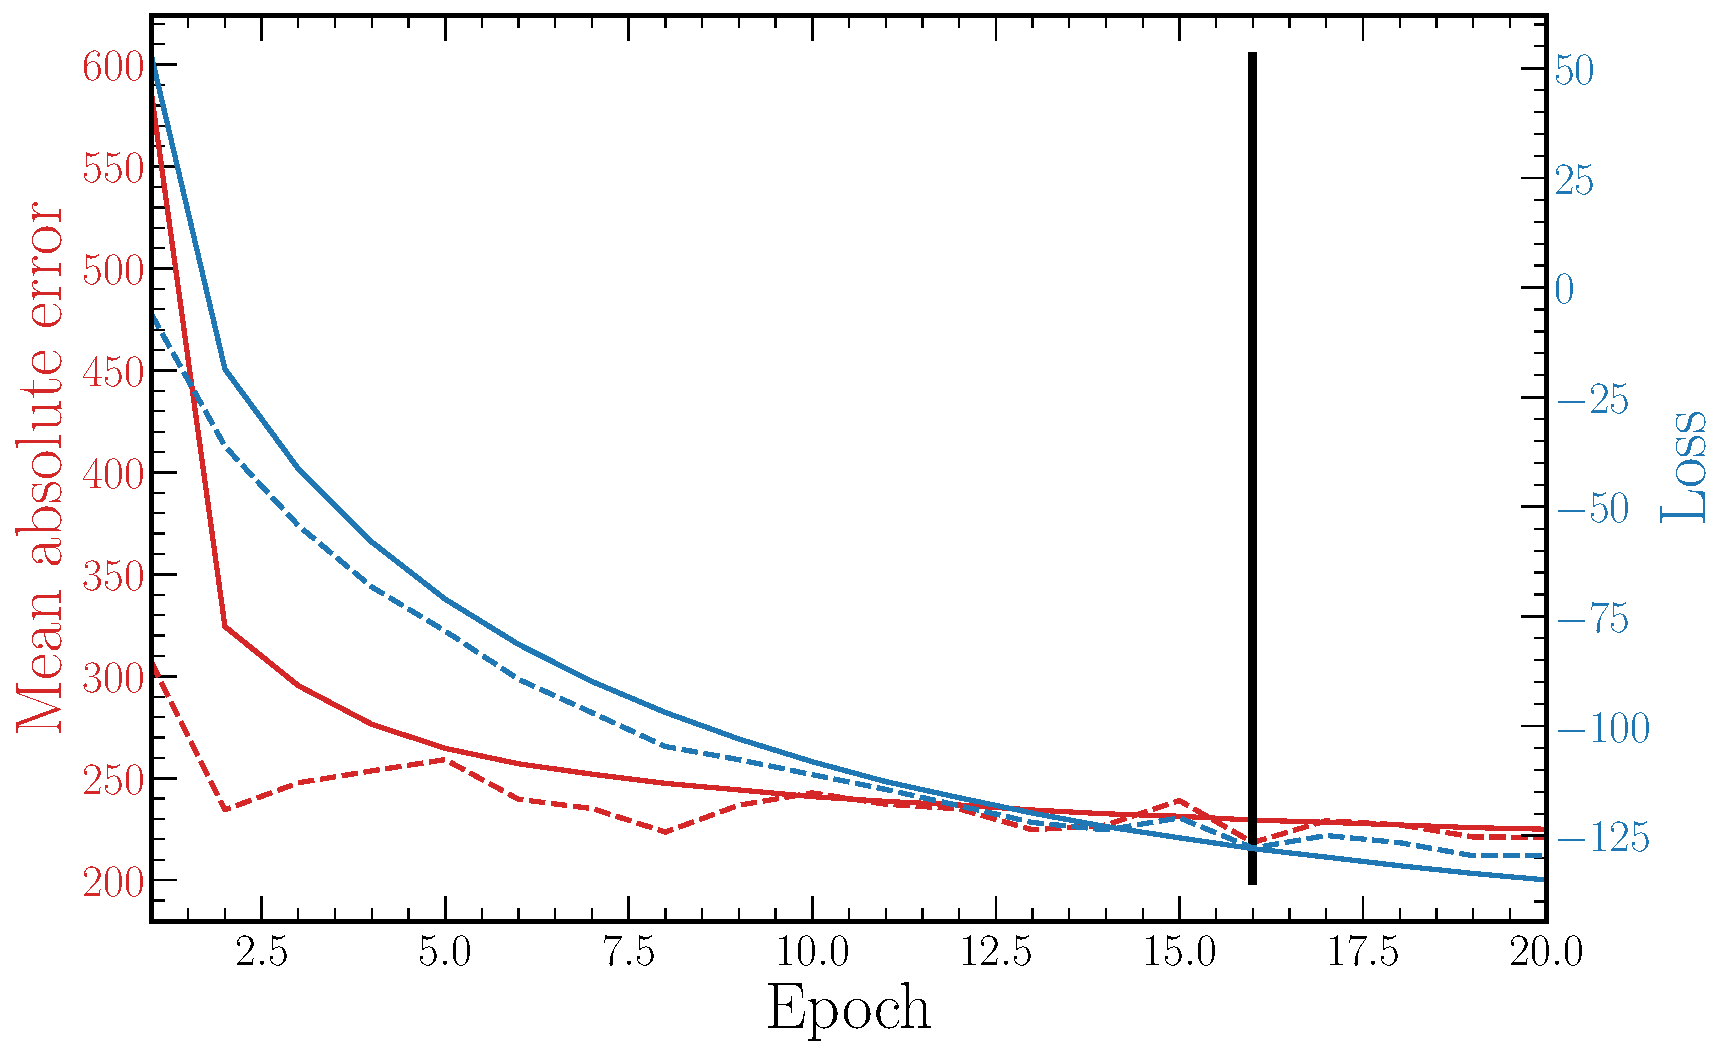
\includegraphics[width=0.7\textwidth]{diagrams/7-results/final_energy_history.pdf}
    \caption[Loss and mean absolute error throughout training for the energy estimation network]
    {Total loss and \emph{neutrino energy} mean absolute error for both the training dataset
        (solid) and validation dataset (dashed) throughout training for the energy estimation
        network trained on CC-QEL and CC-MEC $\nu_{e}$ events. The final network weights are taken
        at epoch sixteen as shown by the vertical black line.}
    \label{fig:final_energy_history}
\end{figure}